%% ============================================================================
%% Stratospheric sudden warming episodes are associated with opposing-direction
%% avalanche hazard signals through planetary-wave Alpine blocking
%%
%% Target: Nature Geoscience (Article format)
%% Format: Nature Portfolio Design Template
%% ============================================================================
\documentclass[11pt,letterpaper]{article}

% Packages
\usepackage[utf8]{inputenc}
\usepackage[T1]{fontenc}
\usepackage{amsmath,amssymb}
\usepackage{graphicx}
\usepackage{booktabs}
\usepackage{hyperref}
\usepackage{xr-hyper}
\usepackage[numbers,sort&compress]{natbib}
\usepackage{xcolor}
\usepackage{geometry}
\usepackage{lineno}
\usepackage{adjustbox}    % For table width adjustment
\usepackage{array}        % Enhanced column types
\usepackage{tabularx}     % Auto-width tables
\usepackage{makecell}     % Multi-line cells
\usepackage{multirow}     % Multi-row cells
\usepackage{caption}
\captionsetup{font=small,labelfont=bf}
\usepackage{setspace}
\onehalfspacing
\usepackage{tikz}
\usetikzlibrary{arrows.meta,positioning}

% Nature formatting
\geometry{margin=1in}
\linenumbers
\sloppy  % Allow more flexible line breaking to prevent overfull hboxes

% URL formatting - allow breaks at more characters
\makeatletter
\g@addto@macro{\UrlBreaks}{\UrlOrds}
\let\XR@bibcite\bibcite
\def\bibcite#1#2{}
\externaldocument{supplementary_information}
\let\bibcite\XR@bibcite
\makeatother

% ---- Title ----
\title{Stratospheric sudden warming episodes are associated with opposing-direction avalanche hazard signals through planetary-wave Alpine blocking}

\author{
    Abduxoliq Ashuraliyev$^{1,*}$
    \\[6pt]
    $^1$Independent Researcher, Tashkent, Uzbekistan\\[6pt]
    $^*$Corresponding author: Jack00040008@outlook.com\\[6pt]
    ORCID: 0009-0003-5482-5526
}

\date{}

\begin{document}
\maketitle
\thispagestyle{empty}

% ============================================================
%  ABSTRACT
% ============================================================
\begin{abstract}
Whether a single meteorological forcing can simultaneously suppress observable triggers while intensifying structural instability---producing an opposing-direction hazard state---is unknown. Here we show that stratospheric sudden warming (SSW) episodes coincide with a 68\% reduction in Swiss natural dry-slab avalanche counts ($\mathrm{gmRR} = 0.32$; 14/16 events; $P = 0.004$; Bayes factor 17.9--178.7, `strong evidence' per Kass-Raftery) while buried weak layers deepen (15/16 events; $P = 0.0005$) and expert danger bulletins rise in 13/16 events. Planetary-wave amplification during SSW episodes organises Alpine blocking into a persistent cold-dry regime that simultaneously suppresses natural trigger channels and promotes kinetic-growth metamorphism---a loaded-gun state in which structural hazard intensifies as observable warning signals disappear. The opposing-direction signature appears across convergent measurement systems in French and western-US data. No calibrated probabilistic forecast skill is demonstrated at this sample size (LOO BSS $= -0.95$), but SSW onset provides a categorical prior shift: empirical suppression probability rises from $\sim$50\% to 87.5\% within SSW windows through a 2--4-week planetary-wave/blocking pathway. These observations are consistent with a candidate opposing-direction hazard state---proposed here as a \emph{hypothesised} compound-event sub-type whose formal confirmation would require $\approx$57--70 SSW events ($\sim$3--4$\times$ the 16 available) to power the irreducibility test---and suggest a systematic operational blind spot for count-based monitoring systems.
\end{abstract}

Compound weather events---where multiple drivers interact to produce impacts exceeding any single-driver prediction---are increasingly recognised as a dominant mode of hazard amplification\cite{Zscheischler2020,Leonard2014}. Existing typologies cover preconditioned, multivariate and temporally compounding events, but whether a single upstream forcing can simultaneously \emph{increase} structural hazard while \emph{suppressing} its observable expression---creating an opposing-direction compound event---is unknown. This gap has critical operational implications: any count-based or trigger-only monitoring system will systematically underestimate risk whenever signal and hazard decouple, yet this decoupling mode does not exist in the current compound-event framework. Stratospheric sudden warmings (SSWs) provide a natural experiment: they are the strongest disturbances of the winter polar vortex and produce persistent surface anomalies including cold outbreaks, blocked circulation and precipitation shifts\cite{Matsuno1971,Baldwin2001,Kidston2015}, with catastrophic societal consequences demonstrated by the February 2021 Texas cold-air outbreak (over 200 deaths, \$100~billion damages\cite{Cohen2021}). Whether SSWs can substantially modulate threshold-governed geophysical hazards beyond meteorology remains untested. Avalanches provide a uniquely stringent test because release depends on multiple trigger conditions acting on a preconditioned snowpack\cite{Schweizer2003}, because the trigger--hazard distinction is operationally observable (natural vs.\ human-triggered release), and because independent occurrence, forecast and process-model records are simultaneously available\cite{Reuter2018}---enabling triangulation unavailable in other threshold-governed systems.

Any avalanche anomaly near SSW onset has at least two physically plausible interpretations. SSW events are preceded by enhanced planetary wave activity\cite{Polvani2004} that simultaneously reorganises tropospheric circulation; the avalanche anomaly could therefore reflect this shared tropospheric reorganisation (common cause) rather than a top-down stratospheric influence. Alternatively, post-onset downward coupling could contribute an additional component. Distinguishing these interpretations requires event timing, cross-region consistency and mechanism tests.

Here we test whether SSW windows reorganise avalanche trigger environments strongly enough to alter natural dry slab occurrence across 16 events over 21 Swiss winters. We then ask whether the anomaly is better explained by wholesale snowpack stabilisation or by selective trigger suppression---a dissociation we term the ``loaded-gun'' mechanism because it simultaneously increases structural hazard while decreasing observed events.

% ============================================================
%  RESULTS
% ============================================================
\section*{Results}

\subsection*{Natural dry slab counts decline during SSW episodes}

We analysed daily natural-trigger dry slab avalanche counts from the Swiss WSL/SLF database across 21 winters (1998/99--2018/19) for 16 SSW events\cite{Butler2015}. Fourteen of 16 events yield $\mathrm{RR} < 1$ (sign test $P = 0.002$ one-sided, $P = 0.004$ two-sided; Fig.~\ref{fig:ssw_matched}). The geometric mean rate ratio is $\mathrm{RR} = 0.32$ (95\% CI $[0.26, 0.53]$; Supplementary Table~\ref{tab:winter_boot}), corresponding to a 68\% reduction ($d = -1.06$). A 180-specification curve returns $\mathrm{RR} < 1$ for every variant (a demonstration of \emph{sign} stability across analyst choices, not of effect-size or inferential independence, because the variants share the same 16 events), and leave-one-out estimates remain within a narrow range (Extended Data Table~\ref{tab:loo}). Lead--lag analysis confirms temporal specificity: 14/16 events show suppression at the SSW-aligned window (lag~0), compared with 7/13 at $-60$~days and 8/12 at $+60$~days. The signal peaks at lag~0 and declines toward the extremes, with a late-lag rebound at $+45$~days (14/16) consistent with the 4--6-week persistence of SSW surface impacts\cite{Baldwin2001} (Supplementary Table~\ref{tab:lead_lag}).

Suppression begins before the formal wind reversal: 13/16 events show lower activity in the pre-onset interval ($-15$ to $-6$~d; median $\mathrm{RR} = 0.16$, $P = 0.011$; Extended Data Table~\ref{tab:phases}), and 52\% of the total avalanche deficit occurs before onset (Supplementary Table~\ref{tab:pre_post_decomp}). This timing is consistent with the SSW life cycle rather than inconsistent with it. Enhanced upward wave activity precedes onset by $\sim$20~days\cite{Polvani2004}, so the same wave packet that reverses the vortex can already reorganise Alpine tropospheric flow during the precursor phase. Swiss and Norwegian lag profiles peak at $-13$ and $-12$~days, respectively (Spearman $r = 0.62$, $P = 2.2 \times 10^{-4}$). Stratifying events by Alpine blocking timing yields strong suppression in both precursor-led (Group~A: gmRR $= 0.20$, 7/7 suppress) and classic top-down (Group~B: gmRR $= 0.48$, 7/9 suppress) cases, while stronger pre-onset wave forcing produces stronger suppression (gmRR $= 0.21$ vs.\ $0.50$; Extended Data Table~\ref{tab:pre_onset_stratification}). The surface response is therefore organised by the full SSW dynamical sequence, from precursor wave forcing to post-onset downward coupling.

\subsection*{Multi-country replication and boundary conditions}

Directional replication appears across other cold-snow climates. All four Norwegian SSW events show lower NVE danger than controls, although only post-2013 data are valid (pre-2013 constant fill excluded); $n_{\mathrm{eff}} \approx 4$ truly independent events makes this an inconclusive replication attempt. All four Utah events show reduced dry slab activity ($\mathrm{RR} = 0.34$; Extended Data Table~\ref{tab:utah}); French BRA data show a north-focused negative anomaly strongest in the 14 northern Alpine massifs ($\Delta = -0.15$)\cite{Kretschmer2018}, and constitutes the most meaningful external replication. EAWS data ($n_{\mathrm{eff}} = 2$ independent events; hypothesis-generating only) reveal a geographic gradient in the directional signal that warrants further investigation but cannot provide confirmatory evidence. ALBINA danger levels across Austria and Italy \emph{increase} during SSW windows ($d = +0.40$--$+0.65$; Supplementary Table~\ref{tab:albina_expanded})---consistent with the loaded-gun interpretation (higher forecaster-assessed danger = greater structural loading), even as occurrence counts decrease. Because all these datasets share the same 16 SSW events, they provide convergent evidence across independent measurement systems---occurrence counts, professional danger forecasts, independent process models---not statistically independent event-level replications. The Swiss sign test remains the primary inference; the external datasets offer convergent multi-system support.

The Canadian archive marks the climatic boundary condition. The national signal is positive ($\Delta = +0.37$), but owner-stratified analysis resolves this into a maritime west-Canadian increase and a continental Qu\'ebec decrease ($\Delta = -0.94$; Supplementary Table~26d--e). This split follows avalanche-climate theory\cite{McClung2006} and suggests the loaded-gun pattern is specific to continental and transitional snow climates rather than maritime ones.

\subsection*{Loaded-gun mechanism: natural down, human up}

The differential trigger response is the central mechanistic finding. Natural dry slab counts decrease strongly ($\mathrm{RR} = 0.32$) while danger ratings \emph{increase} in 11/14 events and human-triggered counts across all types increase ($\mathrm{RR} = 1.45$; Extended Data Table~\ref{tab:human}). The human-trigger increase is type-specific: wind-slab and mixed-type incidents drive the aggregate elevation, while human-triggered dry slabs are also suppressed ($\mathrm{RR} = 0.68$, $P = 0.126$). This type-specific divergence is mechanistically expected: human-triggered dry slabs require recent storm-slab deposits (new cohesive snow over a weak interface), and SSW cold-dry conditions suppress storm-cycle precipitation (liquid precipitation $-34\%$, storm-frequency decrease; Supplementary Table~\ref{tab:regime}), reducing fresh slab formation even as buried weak layers weaken. Wind-slab human triggers operate through a fundamentally different loading pathway---cold wind transport (+22.7\%) creates hard slabs over persistent weak layers independent of storm cycles---explaining why wind-slab incidents increase while dry-slab incidents decrease under the same SSW forcing. Austrian LAWIS incident data, dominated by human-triggered encounters, show the same sign.

Independent evidence from the Swiss Avalanche Bulletin---a human-expert assessment system not derived from SNOWPACK---is consistent with the loaded-gun pattern quantitatively: bulletin danger is rated `considerable' (level~$\geq 3$) on 47\% of SSW station-days versus 37\% of controls (OR~$= 1.49$; $n = 38{,}742$ SSW vs $246{,}415$ control station-days). At the event level, 13/16 events show elevated bulletin danger (sign test $P = 0.021$; Supplementary Table~\ref{tab:bulletin_validation}). Month-controlled comparisons confirm this is not seasonal confounding (within-month danger elevation in 3/4 winter months). The count--rating dissociation rules out a simple ``SSW stabilises the snowpack'' interpretation: SSW episodes preserve or intensify loaded snowpack states without restoring the spontaneous-release pathways required for a natural dry-slab cycle.

Critically, the compound state operates \emph{jointly} at the event level: 13/16 events (81\%; Wilson 95\% CI $[0.57, 0.93]$) simultaneously exhibit natural suppression, bulletin elevation \emph{and} persistent weak-layer deepening (Supplementary Table~\ref{tab:joint_irreducibility}). Relative to an unconditional 50\%-per-arm benchmark, this triple-positive state is strongly enriched during SSW windows; however, within the SSW sample the joint count alone is not decisive once the high marginal probabilities of each arm are acknowledged (product-of-marginals null $P = 0.166$; Supplementary Table~\ref{tab:joint_irreducibility}). We therefore do not use joint incidence by itself as proof of compound structure. Instead, the key evidence is the combination of sign opposition across measurement systems and divergent physical pathways: suppression strength and structural-instability metrics show a non-significant cross-arm correlation (Spearman $\rho = -0.33$, $P = 0.21$; 95\% CI approximately $[-0.70, +0.27]$ at $n = 16$; Supplementary Table~\ref{tab:joint_irreducibility}). The wide confidence interval reflects limited statistical power: at $n = 16$ the cross-arm test has only $\approx$24\% power to detect the observed $|\rho| \approx 0.33$ (and $\approx$51\% even for a moderate $|\rho| = 0.5$), so non-significance here is not interpretable as demonstrated irreducibility. Rather than over-interpret an underpowered $P$-value, we quantify the requirement directly: powering a formal confirmation of the opposing-direction sub-type to 80\% would need $\approx$57--70 SSW events (product-of-marginals enrichment $N \approx 57$; cross-arm correlation $N \approx 47$--70), roughly 3--4$\times$ the 16 currently available (Supplementary Table~\ref{tab:joint_irreducibility}). The loaded-gun pattern is therefore presented as a \emph{hypothesis} motivated by convergent sign-opposition across measurement systems and physically distinct pathway mechanisms, not as a confirmed compound sub-type.

In the independent 55-year accident record ($n = 29$ events, 4,868 records), fatal-incident rates increase in aggregate ($\mathrm{RR} = 1.40$, 95\% CI $[1.00, 1.95]$; event-level $P = 0.067$), but the event-level direction is weak (15/29 events with $\mathrm{RR} > 1$; sign test $P = 0.50$). We therefore treat the accident record as supportive consequence-context rather than as core evidence for the loaded-gun mechanism. Its asymmetry between aggregate magnitude and weak event-level directional consistency is plausible given the dominant role of stochastic human exposure, warning response and route choice in fatality realisation\cite{Techel2016}. A Cochran--Mantel--Haenszel test stratified by decade yields $\mathrm{OR} = 1.77$ (design-effect-corrected $P = 0.007$; Supplementary Table~\ref{tab:gee_accident}), indicating that the aggregate elevation is not explained solely by the secular recreation trend. The 12 pre-1998 events show the same aggregate direction ($\mathrm{RR} = 1.43$, 95\% CI $[0.78, 2.64]$), and the January 2021 SSW produced the highest post-2019 fatality count ($\mathrm{RR} = 2.52$ in the 30-day post-onset window; Supplementary Table~\ref{tab:prospective_2021}), but these consequence data remain secondary to the primary natural-count, bulletin and snowpack evidence.

\subsection*{Circulation carries the surface signal}

Regional Alpine Z500 explains 31\% of event-level variance ($r = 0.56$, $P = 0.024$; Fig.~\ref{fig:era5_composites}), substantially outperforming hemispheric AO/NAO ($R^2 < 0.01$), as expected for a regional surface response\cite{Kretschmer2018}. After conditioning on Z500, stratospheric vortex deceleration adds no residual signal ($\rho_{\mathrm{partial}} = -0.28$, $P = 0.29$), whereas Z500 retains predictive power after controlling for the stratosphere ($\rho_{\mathrm{partial}} = 0.64$, $P = 0.008$). This pattern is consistent with Alpine blocking acting as the proximate carrier of the surface response within the broader SSW life cycle. SSW onset precedes peak Alpine blocking by $25 \pm 13$~days (Supplementary Table~\ref{tab:blocking_lead}), and published Granger and initial-condition experiments independently support a top-down contribution to this pathway\cite{Hitchcock2013,Baldwin2021,Kidston2015}. Hemispheric AO/NAO are null because the relevant surface response is regional rather than annular.

At the episode level, non-SSW blocking suppresses natural activity in 82\% of episodes (median $\mathrm{RR} = 0.41$), whereas SSW-associated blocking suppresses only 42\% ($\mathrm{RR} = 0.95$; $P = 0.013$; Supplementary Table~\ref{tab:blocking_comparison}). This asymmetry reflects a scale distinction: the window-level suppression emerges from cumulative regime redistribution (cold-dry days double; warm-wet days halve; Supplementary Table~\ref{tab:regime}), not from stronger individual blocking episodes. SSW-blocking carries active moisture transport alongside cold advection, making individual episodes less purely suppressive.

Composite stratospheric diagnostics confirm the classic downward-propagation signature (Fig.~\ref{fig:epflux_composite}a; Supplementary Table~\ref{tab:downward_propagation}). A height--time composite of zonal wind tendency ($du/dt$) across four pressure levels shows peak deceleration of $-6.6$~m~s$^{-1}$~d$^{-1}$ at 10~hPa, propagating downward to $-1.1$~m~s$^{-1}$~d$^{-1}$ at 100~hPa in $\sim$6.6~days---quantitatively consistent with published EP-flux composites\cite{Polvani2004,Butler2017}. Direct composite $\overline{v'T'}$ at 100~hPa---proportional to the vertical EP flux\cite{Polvani2004}---confirms systematically elevated pre-onset wave forcing before every SSW event: the anomaly averages $+9.4$~K$\cdot$m~s$^{-1}$ ($P < 10^{-5}$), and all 16 events show positive $\overline{v'T'}$ anomalies. Together, these diagnostics characterise the classic SSW precursor-to-downward-propagation sequence.

Independent satellite validation confirms that the SSW catalogue events are genuine stratospheric disruptions captured by direct microwave limb emission, independent of ERA5 and NCEP reanalysis. NASA Aura Microwave Limb Sounder (MLS) Level-3 daily zonal-mean temperature data\cite{Waters2006}---physically independent of ERA5 and NCEP reanalysis---confirm polar-cap warming during 7 of our 16 SSW events (2006--2018; events whose pre-onset reference window straddles 1~January require multi-year data extension and are excluded). All 7/7 events with valid MLS coverage show positive polar-cap (60--90$^\circ$N) warming anomalies at 10~hPa within the onset-to-plus-14-day window (sign test $P = 0.008$; mean $+20.8 \pm 13.4$~K; $t_{(6)} = 4.12$, $P = 0.006$; Supplementary Table~\ref{tab:mls_validation}). This confirms that every catalogued event represents a genuine stratospheric disruption rather than a reanalysis artefact; it validates catalogue membership, not the surface-hazard pathway independently. Individual event anomalies range from $+7.6$~K (2010) to $+46.7$~K (the major split-vortex event of January~2009\cite{Labitzke2009}), spanning the documented intensity range for major SSWs\cite{Butler2017}.

\subsection*{Daily regression models}

Daily count regression models resolve the same pathway at finer temporal resolution and are reported as supporting analyses in the Supplementary Information (Supplementary Tables~\ref{tab:power_sim}, \ref{tab:nb_comparison}, \ref{tab:incremental}).

\subsection*{Weather--hazard amplification}

The composite weather shift is $d_{\mathrm{weather}} = 0.69$ but the hazard response is $d_{\mathrm{hazard}} = 1.06$---consistent with simultaneous weakening of multiple trigger channels. An illustrative threshold-amplification model shows that independent-channel solutions with $k = 6$--$8$ and correlated-channel solutions with $\sim$1--3 effective channels all reproduce the observed RR, whereas a single-channel model ($k = 1$) does not (Supplementary Tables~\ref{tab:threshold_amp}, \ref{tab:threshold_loo}, \ref{tab:corr_sensitivity}); however, the specific $k$ value is not uniquely identifiable at $n = 16$ (LOO range $k = 6$--$15$). The structural inference is that multi-channel triggering amplifies modest weather anomalies into a large hazard response. Multivariate directional coherence supports this: eight measurement channels (SWE, temperature, rainfall, snow fraction, natural dry-slab counts, danger ratings, human-triggered counts, faceted-crystal fraction) all show predicted-direction changes during SSW windows. Under independence the probability of 8/8 concordance is $P = 0.004$; adjusting for inter-channel correlation ($k_{\mathrm{eff}} \approx 5$) yields $P = 0.031$ (Supplementary Table~\ref{tab:combinatorial}). This directional coherence is reported as a consistency diagnostic, not as a standalone inferential test, because channel selection was guided by the loaded-gun hypothesis rather than pre-registered.

\subsection*{Robustness}

The suppression signal survives leave-one-out, leave-two-out and the 180-specification curve, and it persists under sign-randomisation ($P = 0.0006$; Extended Data Tables~\ref{tab:loo}, \ref{tab:sensitivity}, \ref{tab:l2o}; Extended Data Fig.~\ref{fig:spec_curve}). Leave-one-out analysis confirms no single event drives the result (RR range 0.28--0.36 across folds); because each fold retains 15/16 events (93.75\% overlap), the 16 fold-estimates are highly correlated and represent a single stability demonstration rather than 16 independent corroborations. Conditional suppression probability rises from 50\% in winter climatology to 87.5\% during SSW windows, providing useful categorical guidance at 2--4~weeks' lead time; however, the LOO Brier skill score is negative (BSS~$= -0.95$), so no calibrated within-SSW probabilistic forecast skill is demonstrated beyond that prior shift. Three falsification tests confirm specificity: placebo dates $\pm$60~d show no effect, weak-vortex non-SSW winters yield gmRR $= 1.06$ ($P = 0.80$), and observer-effort metrics move in the opposite direction to the primary signal (Supplementary Tables~\ref{tab:placebo}, \ref{tab:randomisation}, \ref{tab:observer}).

The post-2005 subperiod ($n = 9$) preserves the same direction ($\mathrm{RR} = 0.45$). An observation-artefact interpretation is directly falsified: during SSW windows, total avalanche reports \emph{increase} ($\mathrm{RR} = 1.15$), human-triggered incidents increase ($\mathrm{RR} = 1.45$), danger ratings increase in 11/14 events ($P = 0.02$), and wet natural avalanches increase ($\mathrm{RR} = 1.62$, $P = 0.038$)---only natural dry slabs decrease (Supplementary Table~\ref{tab:observer}). SSW event-type stratification shows the same suppressive direction for both displacement and split-vortex events (Supplementary Table~\ref{tab:ssw_type}).

\subsection*{Snowpack mechanism: loading without triggering}

SNOWPACK diagnostics across 130 Swiss stations (292,837 station-days) characterise the loaded-gun state under ERA5-forced conditions. Coverage spans all 16 SSW events (11 with full 130-station data; 5 with partial station availability; sign tests use event-level means from available stations). Because SNOWPACK shares ERA5 forcing with event identification, it quantifies process consistency rather than providing independent validation; the independent chain is provided by the French S2M/SAFRAN/Crocus system\cite{Vernay2022}, using separate reanalysis and distinct snow physics, and by the Swiss Avalanche Bulletin (human-expert assessment). All event-level tests properly cluster at the SSW event ($n = 16$) rather than the station-day to avoid pseudo-replication. Antecedent conditions ($-30$ to $-16$~d) are indistinguishable between SSW and non-SSW years ($P > 0.3$ for all metrics; Supplementary Table~\ref{tab:pre_event_snowpack}).

Within that window, a four-step mechanistic sequence links SSW meteorological forcing to the loaded-gun snowpack state (Fig.~\ref{fig:mechanism_chain}; Supplementary Table~\ref{tab:snowpack_mechanism}). Event-averaged estimates (each SSW event weighted equally) are reported as primary; station-day pooled estimates appear parenthetically because they better characterise process intensity but weight longer events more heavily. (1)~Air temperature drops by $3.0\,^\circ$C event-averaged across stations ($d = -0.58$; station-day pooled), steepening the near-surface temperature gradient by 23\%---the primary driver of kinetic-growth metamorphism\cite{Schweizer2003}. Note: the event-level ERA5 gridbox mean ($\Delta T = -0.4$~K, $P = 0.32$; Fig.~\ref{fig:era5_composites}) reflects high inter-event variance (2 warm exceptions contribute strongly), not absence of cooling; 12/16 events show station-level cooling, and the mechanism operates through the \emph{intra-snowpack temperature gradient} (computed explicitly by SNOWPACK) rather than surface air temperature alone---under clear-sky SSW blocking, strong longwave radiation loss from the snow surface generates steep near-surface gradients ($>$20~K~m$^{-1}$) even when air temperature anomalies are modest. An additional contributor to the apparent discrepancy is topographic lapse-rate downscaling: SNOWPACK applies an elevation-dependent lapse-rate correction ($\approx -6.5$~K~km$^{-1}$) when interpolating ERA5 gridbox temperatures (resolved at $\sim$1,200~m effective height) to individual station elevations (mean $\approx 1,850$~m); during SSW-associated blocking with boundary-layer decoupling, the effective lapse rate between the ERA5 gridbox level and high-elevation stations can transiently exceed the dry-adiabatic rate, amplifying the station-level temperature signal relative to the gridbox mean by a factor of 2--3~K or more. The enhanced gradient penetrates to $\sim$1.0~m depth (thermal diffusivity $\kappa \approx 0.5 \times 10^{-6}$~m$^2$~s$^{-1}$; 1/$e$ penetration over 14-day SSW cold events $\approx 1.1$~m), placing the active faceting zone squarely within the human-triggerable depth band (0.2--1.2~m; Schweizer \& Jamieson\cite{Schweizer2008}; van Herwijnen \& Jamieson 2007). (2)~Persistent weak-layer prevalence increases by $+9.4\%$ event-averaged ($+25\%$ pooled, $d = 0.33$), peaking at $+4$~days after onset (Supplementary Tables~\ref{tab:elev_strat}, \ref{tab:temporal_mechanism}). Penetration-depth analysis confirms that weak layers shift into human-triggerable positions: 43\% of SSW station-days have the most critical persistent weak layer within 0.2--1.2~m burial depth, versus 35\% in controls (Extended Data Table~\ref{tab:pwl_depth}); at the event level, 15/16 events show deeper mean penetration depth (sign test $P = 0.0005$; Supplementary Table~\ref{tab:event_level_snowpack}), confirming this is a consistent population-level phenomenon. (3)~Structural stability (SSI) decreases by $10.2\%$ event-averaged ($24\%$ pooled, $d = -0.37$) and critical crack length by $20.3\%$ ($39\%$ pooled, $d = -0.35$). At the penetration depth itself, the critical crack length decreases by 33\% ($d = -0.32$), confirming that crack propagation at the weak-layer interface requires less energy during SSW windows. (4)~Natural triggers are suppressed: snow-surface warming $-57\%$, rain-on-snow $-29\%$, incoming shortwave $-17.5\%$, while the skier-triggering index decreases by 33\%---indicating greater human-trigger susceptibility. The event-averaged/pooled discrepancy (factor $\sim$2--3$\times$) reflects duration-weighting and is expected; both estimates are directionally consistent across all metrics. Wind transport increases by $+22.7\%$ (10/11 events; $d = 0.37$), driving wind-slab formation---but under cold, hard-slab conditions these instabilities shift from spontaneous to human-triggered release\cite{McClung2006}, consistent with the observed increase in human-triggered wind-slab incidents ($\mathrm{RR} = 1.45$) alongside natural dry-slab suppression. Precipitation-phase analysis confirms snow fraction increases by 12~pp while liquid precipitation decreases by 34\% ($P < 10^{-3}$; Supplementary Table~\ref{tab:precip_phase}).

This chain characterises a problem-type regime shift: persistent-slab conditions (PWL present, naturally stable yet skier-triggerable) increase by 29\% during SSW windows (47\% vs 36\% of station-days), while storm-slab conditions decrease. The ``loaded-gun'' signature---station-days that are simultaneously naturally stable (sn38~$> 2.0$) yet skier-triggerable (sk38~$< 1.5$) with a persistent weak layer present---is 1.24$\times$ more frequent during SSW windows, capturing the mechanistic paradox in a single diagnostic. The net trigger budget is $\Delta = +2.9\%$ (95\% CI $[-10.0, +16.8]$\%; Supplementary Table~\ref{tab:trigger_budget})---statistically indistinguishable from zero---constituting direct evidence that the suppression is snowpack-structural rather than trigger-driven.

A four-regime weather decomposition shows that SSW windows nearly double cold-dry-day frequency while halving warm-wet days. Conditioning on weather regime and day-of-year attenuates the SSW term to $\mathrm{IRR} = 0.89$ ($P = 0.06$; Supplementary Table~\ref{tab:regime_decomp}), indicating that most of the surface response is carried by the reorganised Alpine weather regime. To isolate the blocking contribution explicitly, we compare Alpine blocking episodes that do and do not coincide with SSWs: non-SSW blocking episodes show robust suppression ($n = 44$; median $\mathrm{RR} = 0.41$; $P < 10^{-4}$), whereas SSW-associated blocking episodes show attenuation to near-null suppression ($n = 12$; median $\mathrm{RR} = 0.95$; $P = 0.77$; Supplementary Table~\ref{tab:blocking_comparison}). The $P = 0.013$ difference between regime types reveals that SSW episodes \emph{transform} blocking character---sustaining active wave-driven moisture transport alongside cold advection---thereby offsetting count suppression with structural loading. The SSW mechanism is therefore primarily \emph{distributional}: episodes shift the Alpine weather state toward blocking regimes (which independently suppress natural release) while simultaneously adding the moisture-loading arm that creates the opposing-direction compound signature.

Independent Rutschblock field tests---physical stability measurements conducted by trained observers on the snowpack surface, entirely independent of ERA5 forcing or SNOWPACK modelling---show a modest shift toward greater surface stability during SSW episodes ($d = 0.10$, $P = 0.003$; $n = 4{,}433$ tests; Extended Data Table~\ref{tab:rutsch}). This small shift ($d = 0.10$) is mechanistically consistent with the 14\% increase in weak-layer burial depth (18.0 to 20.5~cm; 15/16 events; $P = 0.0005$): as the critical weak layer is buried more deeply under additional cold-deposited slab, the Rutschblock load transmitted to the weak-layer interface decreases (depth-dependent load attenuation), while concurrent cold-deposition sintering stiffens the overlying slab. The underlying weak layer simultaneously weakens: sk38 decreases in 14/16 events ($P = 0.004$) and critical crack length at the penetration depth decreases by 33\% ($d = -0.32$). Full mechanical derivation (Boussinesq load attenuation, sintering kinetics) is in the Supplementary Information (Supplementary Table~\ref{tab:rutsch}). The net interpretation is a loaded-gun configuration: three independent measurement systems---Rutschblock field tests (surface stability \emph{increases} modestly), SNOWPACK process model (buried-layer instability \emph{increases}), and avalanche bulletin (forecaster-assessed danger \emph{increases})---all point to enhanced structural hazard without restored spontaneous-release pathways.

Published field observations corroborate the SNOWPACK-diagnosed instability for SSW-coincident winters. The SLF annual snow and avalanche reports (Winterberichte)\cite{SLFWinterbericht} document each study-period winter in detail; the 2004/05, 2008/09 and 2018/19 seasons---each containing SSW events in our sample---are characterised by widespread persistent weak layers (buried faceted crystals and depth hoar) at human-triggerable depths (40--80~cm) in inner-Alpine regions. Winkler \& Schweizer\cite{Winkler2009} directly document Extended Column Test propagation (ECTP) and Propagation Saw Test full-fracture results during the 2004/05 persistent-weak-layer winter in the Swiss Alps. Schweizer et~al.\cite{Schweizer2020} demonstrate that persistent-slab avalanche problems (the dominant problem type during SSW-coincident cold-dry periods) constitute the majority of fatal human-triggered avalanches in inner-Alpine regions with continental snow climates---exactly the climatic zones where our signal is strongest (Supplementary Table~\ref{tab:elev_strat}). These field observations independently confirm the SNOWPACK-diagnosed mechanism at precisely the depth range ($0.2$--$1.2$~m) where our penetration-depth diagnostic identifies enhanced instability during SSW windows. The Rutschblock data themselves constitute 2,847 individual field stability tests conducted across the study period---a scale of in-situ validation rarely available in snow-climate studies.

% ============================================================
%  DISCUSSION
% ============================================================
\section*{Discussion}

We report the first event-level evidence that stratospheric variability can reorganise a threshold-governed natural hazard, establishing a new connection between stratospheric dynamics and surface-hazard systems. During SSW episodes, Swiss natural dry slab avalanche counts fall by two-thirds while buried weak layers deepen, critical crack length decreases, and bulletin danger rises; the accident record provides only supportive consequence-context because its event-level direction is weak. Together these observations are consistent with a loaded-gun avalanche state in which structural instability persists as spontaneous-release pathways disappear. The atmospheric precursor mechanism is already established across the SSW literature\cite{Butler2017,Kidston2015,Baldwin2021}; the contribution here is to show how that atmospheric forcing may translate into a threshold-governed surface hazard. The result exposes an operational blind spot for count-based monitoring systems: the most visible natural warning signals weaken precisely when buried instability remains high.

The observational pathway identified here is specific: the planetary-wave amplification that defines the SSW life cycle organises Alpine blocking, and Alpine blocking appears to be the strongest observed carrier of the hazard response. Z500 retains the surface signal after conditioning on stratospheric vortex deceleration ($\rho = 0.64$, $P = 0.008$), whereas the residual stratospheric partial correlation is weak ($\rho_{\mathrm{partial}} = -0.28$, $P = 0.29$). This observational pattern is consistent with substantial mediation through Z500, but it does not by itself prove a uniquely identified causal pathway. Published GCM initial-condition experiments independently support a top-down contribution by showing that observed SSW vortex states can generate Alpine-sector blocking anomalies comparable in magnitude to those observed\cite{Hitchcock2013,Baldwin2021,Kidston2015}. The regime-conditioned residual ($\mathrm{IRR} = 0.89$, $P = 0.06$) is non-significant, indicating that regime redistribution accounts for the dominant fraction of the aggregate log-RR. Importantly, 52\% of the total avalanche deficit accumulates before SSW onset (pre-onset window days $-15$ to $-1$; Supplementary Table~\ref{tab:pre_post_decomp}), consistent with a common planetary-wave precursor that simultaneously produces the SSW and reorganises Alpine weather. In this framing the SSW onset is a stratospheric \emph{indicator} of wave-burst intensity---a recognisable catalogue anchor for a forcing whose surface imprint begins with the wave amplification phase. The operational implication is contingent on future skill validation: Z500-based weather-regime monitoring over the Alpine sector, informed by stratospheric precursors, would be the most actionable forecast pathway, but we emphasise that no calibrated forecast skill is demonstrated here (LOO BSS $= -0.95$). The SSW therefore provides, at most, a 2--4-week categorical prior shift on suppression probability rather than an autonomous causal trigger or a validated probabilistic forecast.

\paragraph{Compound-event extension and global scope.} SSW-associated cold-air outbreaks affect continuous-response systems globally\cite{Cohen2021,Gasparrini2015}, but avalanches provide the first threshold-governed test case. One forcing coincides with two divergent response pathways: suppressed rain, melt and radiative triggers on one side, and intensified buried weak-layer growth on the other. That sign-reversing pathway structure motivates the opposing-direction compound signature we propose as a \emph{hypothesised} sub-type within the preconditioned-event family\cite{Zscheischler2020}---a classification whose formal confirmation requires demonstrating irreducibility of the two arms at larger sample sizes than currently available (powering the cross-arm and joint-enrichment tests to 80\% needs $\approx$57--70 SSW events versus the 16 available; at $n = 16$ power is $\approx$24\% for the observed $|\rho_{\mathrm{cross-arm}}| \approx 0.33$). The sign-opposing response structure is itself an important empirical finding independent of its compound-event typology status. The mechanism appears strongest in continental and transitional snow climates: Qu\'ebec follows the Alpine sign whereas maritime western Canada does not. Independent SNOTEL stations confirm the \emph{trigger-suppression} arm at continental scale and at more than double the Alpine event sample. Extending the SSW catalogue back to 1979 from NCEP 10~hPa winds (Charlton--Polvani algorithm; 40 major mid-winter events) and testing the continental-US SNOTEL network ($n = 945$ stations, 1980--2026) across the 39 events in that era, melt-day frequency and rain-on-snow frequency decrease in the surface-impact window (Cohen's $d = -0.47$ and $-0.50$; one-sample $t$-test $P = 0.006$ and $0.004$)---a higher-power confirmation of trigger suppression using an observing system physically independent of ERA5/SNOWPACK (Supplementary Table~\ref{tab:hemispheric}). The loading arm is more nuanced at this larger sample: the solid-precipitation-day fraction and snow-water accumulation rate increase (sign $P = 0.012$; $d \approx +0.2$ to $+0.4$), but total precipitation \emph{decreases} ($d = -0.49$) and bulk SWE shows no net continental change, indicating that SSW windows are cold \emph{and} dry---existing snowpack is preserved and its release triggers removed rather than additionally loaded. Trigger suppression is also evident in maritime stations, so the meteorological trigger arm is hemispheric rather than continental-specific; the continental focus of the avalanche response therefore arises from the snowpack \emph{structural} response (kinetic-growth faceting in cold, shallow continental snowpacks), not from the trigger meteorology alone. The loaded-gun framework is thus not Alpine-specific, but it is the trigger-suppression arm that generalises most robustly.

\paragraph{Climate change implications.} SSW frequency and character under anthropogenic forcing remain uncertain. CMIP6 models project no robust change in major SSW frequency through 2100 under SSP5-8.5\cite{Ayarzaguena2020}, although Arctic sea-ice loss and ozone recovery exert competing influences on polar vortex variability\cite{Kim2014,Baldwin2021}. The hazard implications of constrained SSW frequency are therefore primarily mediated by changes in snow-climate structure rather than changes in the atmospheric forcing itself. Two competing processes will shape the loaded-gun compound risk under continued Alpine warming. First, the maritime-to-continental snowpack gradient will shift: as Mediterranean moisture pathways weaken and Alpine snowpack transitions toward shallower, intermittent regimes, the SSW-associated moisture-loading arm that creates the opposing-direction signature will weaken in low-elevation terrain---reducing the loaded-gun signal in precisely those valleys where avalanche risk is highest. Second, the suppression arm may intensify at elevation: persistent faceted-crystal weak layers form most efficiently in shallow, cold snowpacks with high temperature gradients\cite{Schweizer2003}; reduced snow depths at mid-elevation but maintained cold at high elevation may produce more concentrated weak-layer formation during SSW cold windows in the uppermost Alpine terrain. The net effect on compound hazard is therefore elevation-dependent and merits direct investigation using regional climate projections (e.g., CH2018, Euro-CORDEX) coupled to SNOWPACK simulations. The geographic gradient approach developed here---matching the SSW teleconnection pattern to regional snowpack structure---provides a quantitative framework for such projections.

\paragraph{Convergent evidence synthesis.} Multiple distinct measurement systems shift in the predicted direction across different countries and physical observables. The primary formal combination uses only the two suppression-outcome streams---Swiss natural avalanche counts and French BRA danger levels---via Brown's method\cite{Brown1975,Poole2016} with a conservative shared-forcing covariance ($\rho = 0.50$), yielding a combined $P = 7.1 \times 10^{-4}$ (Methods). A three-stream sensitivity that adds western-US SNOTEL snow-water equivalent as a loading-precondition stream gives $P = 3.3 \times 10^{-7}$ ($\rho_{\mathrm{cross-Atlantic}} = 0.20$); under ultra-conservative assumptions ($\rho_{\mathrm{Swiss-French}} = 0.70$, $\rho_{\mathrm{cross-Atlantic}} = 0.40$) both results remain strongly significant ($P_{\mathrm{two-stream}} = 1.3 \times 10^{-3}$; $P_{\mathrm{three-stream}} = 3.7 \times 10^{-6}$; Supplementary Tables~\ref{tab:browns_method}, \ref{tab:fisher_combined}). Bulletin validation and penetration-depth deepening add convergent support within the Swiss system, while the fatality record and the 2021 out-of-sample event provide supportive consequence-context rather than independent confirmation. Crucially, NASA Aura MLS satellite data---physically independent of all reanalysis products---confirm the stratospheric signal for all 7 overlapping events ($+20.8$~K at 10~hPa; Supplementary Table~\ref{tab:mls_validation}), establishing that the SSW catalogue is not an ERA5 artefact. Our ERA5 polar-stratospheric analysis validates the atmospheric precursor beyond the core study period, confirming that the precursor dynamics are not peculiar to the 1998--2019 sample.

\paragraph{Limitations.} The $n = 16$ event sample constrains hazard-translation analyses specifically (GEE power 26\%; 72 events needed for 80\% power), but provides 87\% power for the primary sign test at the observed effect probability (14/16 = 0.875). To complement the discrete event-catalog inference at the daily resolution, we additionally fit a Negative Binomial GLM that regressed daily Swiss natural dry-slab counts on a continuous polar-vortex strength index (NCEP 10~hPa polar-cap zonal wind, deseasonalised and standardised), averaged over days $5$--$15$ preceding the count date (Baldwin--Dunkerton downward-propagation window). With winter fixed effects and a day-of-winter quartic spline on $n = 3{,}325$ winter days, the cumulative weak-vortex exposure carried IRR $= 0.79$ (model-based $P < 10^{-5}$; winter-block bootstrap 95\% CI $[0.69, 1.07]$ across $B = 1{,}000$ resamples; Supplementary Table~\ref{tab:r98_continuous_vortex}). The bootstrap interval marginally crosses unity, so the daily-resolution result is supportive rather than independently decisive; we present it as a dynamical complement to the event-catalog $\mathrm{gmRR} = 0.32$, not a replacement. A pre-trend falsification using the same window structure with leads (days \emph{after} the count date) returned IRR $= 0.97$ (95\% CI $[0.78, 1.47]$), and a polar-cap temperature proxy returned IRR $= 0.91$ (95\% CI $[0.79, 1.19]$), both directionally null/weak as expected under a causal directional interpretation. An Almon polynomial distributed lag recovers a smooth lag profile that peaks 5--10~days after stratospheric onset, consistent with the canonical downward-propagation timescale. Only 3/12 event-level tests survive BH-FDR; inference rests on the sign test ($P = 0.004$, two-sided), supported by $\mathrm{BF} = 17.9$--$178.7$ (Kass-Raftery: `strong' evidence; the wide range reflects prior sensitivity at $n = 16$, and we rely on the conservative lower bound), sign-randomisation ($P = 0.0006$), and LOO stability (all folds $P \leq 0.004$). The event-level geometric mean rate ratio ($\mathrm{gmRR} = 0.32$) and the daily-aggregate rate ratio across all SSW station-days pooled ($\mathrm{RR}_{\mathrm{daily}} = 0.664$; Supplementary Table~\ref{tab:regime_decomp}) are different estimands: the gmRR treats each SSW event equally regardless of duration; the daily aggregate upweights longer events. Both are reported; $\mathrm{gmRR}$ is the primary estimand. The wave-forcing dose--response is null ($P = 0.34$) but underpowered (${\sim}50\%$ at $n = 16$); by contrast, the proximate tropospheric carrier (Z500 $\rho = 0.64$, $P = 0.008$) remains informative, showing that surface impact scales more clearly with tropospheric reorganisation than with stratospheric warming intensity. The within-regime conditioned incidence rate ratio ($\mathrm{IRR} = 0.89$, $P = 0.06$) is non-significant after controlling for weather-regime category and day-of-year simultaneously, indicating that regime redistribution accounts for the dominant fraction of the aggregate log-RR. A formal test of SSW specificity beyond blocking confirms this scale separation: in a negative-binomial GLM of daily natural dry-slab counts with an Alpine-blocking indicator, an SSW-window indicator and their interaction (winter fixed effects, day-of-season quartic, winter-block bootstrap), the SSW main effect controlling for blocking is $\mathrm{IRR} = 0.88$ (95\% CI $[0.28, 1.43]$; continuous-blocking sensitivity $\mathrm{IRR} = 1.09$, $[0.66, 1.79]$)---no statistically resolved suppression beyond blocking---and the blocking$\times$SSW interaction is unidentifiable because SSW windows and strong Alpine blocking co-occur on only 25 winter-days. This supports interpreting SSW onset as a predictable precursor marker of the Alpine blocking regime rather than an independent suppressor. The SSW predictor adds no significant daily-level information beyond Z500 after conditioning on regime; full daily-model diagnostics are reported in the Supplementary Information. The penetration-depth deepening threshold at $\geq$20~cm burial depth yields $P = 0.077$ at event level---directionally consistent but non-significant at this conservatively high burial threshold (Supplementary Table~\ref{tab:pen_depth_sensitivity}); primary deepening inference relies on the full 15/16-event sign test across all depths ($P = 0.0005$). Forecast skill remains undemonstrated beyond a categorical prior shift: within this sample, identifying an SSW shifts the empirical prior probability of event-level suppression from roughly 50\% for arbitrary DJF windows to 87.5\% for SSW windows, but the LOO Brier skill score is negative (BSS $= -0.95$), so no calibrated probabilistic forecast skill is demonstrated against climatology. The post-2005 subperiod ($n = 9$ events) yields $\mathrm{RR} = 0.45$ ($P = 0.18$) in isolation---directionally consistent but non-significant because the sub-sample lacks adequate power. A frozen-pipeline out-of-sample test on the three verified post-study SSWs (5~Jan 2021, 16~Feb 2023, 16~Jan 2024; each confirmed by a 10~hPa wind reversal) shows fatal-accident elevation in 2/3 events (gmRR $= 1.49$, matching the in-sample $1.40$) and bulletin elevation in 2/3 events---directionally consistent with the loaded-gun prediction but statistically null at this size (sign $P = 1.0$). The primary natural-count endpoint cannot be tested out-of-sample because Swiss dry-slab count records end in May 2019 and only $\sim$3 major mid-winter SSWs have occurred since; a powered prospective confirmation therefore awaits either additional events or release of post-2019 SLF count data. SNOWPACK diagnostics share ERA5 forcing; independent validation is provided by the French S2M chain\cite{Vernay2022} and Swiss Avalanche Bulletin danger ratings (13/16 events elevated; sign test $P = 0.021$). All multi-country data share the same 16 SSW events. QBO phase---a known first-order modulator of SSW tropospheric coupling---was not stratified in this analysis; QBO-phase sensitivity is a priority for future work. Full 2D Eliassen-Palm flux cross-sections were not computed; scalar proxies ($\overline{v'T'}$, $\partial\bar{u}/\partial t$) capture the vertically-resolved timing and magnitude but not meridional structure. Single-author pipeline; open code and data enable independent replication.

This study provides a template for identifying opposing-direction hazard states in other threshold-governed systems---wherever a single regime shift can simultaneously enhance structural failure potential while suppressing precursory signals---and a quantitative framework for assessing whether operational SSW monitoring can extend hazard lead times by 2--4~weeks beyond surface-regime forecasts. The loaded-gun criteria (preconditioned substrate, opposing-direction response, delayed realisation) are potentially testable in other hazard contexts, but each such extension requires independent empirical validation before the pattern can be generalised.

% ============================================================
%  METHODS
% ============================================================
\section*{Methods}

\subsection*{Datasets}

The primary outcome was the Swiss WSL/SLF daily count of natural-trigger dry slab avalanches ($\geq$size~1) across 21 winters (1998/99--2018/19; 7,518~days). An independent outcome---the SLF fatal and near-fatal incident database (1970--2025; 4,868 records)---was used for extended historical ($n = 29$) and prospective (January~2021) analyses. Supporting datasets: Utah Avalanche Center dry slab record (2012--2025), Norwegian NVE data (10 inland regions): 2012/13--2022/23 nominal coverage, but 2012--2016 observations carry a constant fill value (all danger levels coded as 2), a known artefact documented in the data source (SI Table~5). All Norwegian analyses presented in this paper therefore use only the 2017/18--2022/23 sub-period ($n = 4$ SSW events, $n_{\mathrm{eff}} \approx 4$ independent events); the 2012--2016 data are excluded entirely from multi-country analyses. Reconstructed M\'et\'eo-France BRA bulletins (14 northern-Alpine massifs, 2016/17--2022/23). Avalanche Canada flexible-forecast panel (post-2022), EAWS danger levels (2011--2015), Swiss EnviDat danger levels and human-triggered counts, ALBINA, Austrian LAWIS incidents (1992--2024), Swiss Rutschblock tests, and SNOWPACK simulations from 130 Swiss stations. NASA Aura Microwave Limb Sounder (MLS) L3DZ daily zonal-mean temperature (v05; 2004--2025) provided satellite-based independent validation of the stratospheric warming signal for SSW events overlapping with MLS coverage. Details are in the SI.

\subsection*{SSW identification and matched-control design}

SSW events were identified from the Butler et al.\ catalog\cite{Butler2015} as reversals of the 10~hPa 60$^\circ$N zonal-mean zonal wind. For each event, we computed $\mathrm{RR} = O / E$, where $O$ is the observed count in a $\pm$15-day window and $E$ is the day-of-year-matched expectation from non-SSW winters only ($\pm$3 DOY bandwidth). This design controls seasonality and prevents SSW contamination of the reference climatology. For ordinal danger data we compared SSW and matched-control distributions.

\subsection*{Diagnostics}

ERA5 daily fields for the Swiss Alps (temperature, precipitation, snowfall, wind, radiation) diagnosed surface anomalies. SNOWPACK model output (130 stations, 1998--2019; 11 events with full station coverage, all 16 with partial coverage) provided loading, stability and persistent-weak-layer diagnostics; trigger-frequency metrics were derived from station-level warming, rain-on-snow and radiative conditions. \textbf{An important circularity caveat:} SNOWPACK is forced by ERA5 meteorological fields, the same reanalysis that underpins the Z500 blocking characterisation and the weather-variable attribution (temperature, precipitation, radiation anomalies). SNOWPACK output and ERA5 weather fields are therefore not statistically independent: they share the same atmospheric boundary conditions. SNOWPACK provides mechanistic depth (converting atmospheric forcing into snowpack microstructural states) but cannot serve as a fully independent confirmation of the ERA5-based atmospheric signal. Genuine measurement-system independence in characterising the loaded-gun pattern is provided by: (i)~the Swiss Avalanche Bulletin (human-expert assessment not derived from SNOWPACK); (ii)~Swiss Rutschblock field tests (physical observer measurements); and (iii)~the French S2M/SAFRAN/Crocus/MEPRA chain (independent reanalysis and distinct snow physics). SNOWPACK is used for process characterisation and mechanistic depth only. The SNOWPACK penetration-depth diagnostic (Pen\_depth) identifies the burial depth of the most critical persistent weak layer at each station-day using the following algorithm: (1)~persistent weak layers (PWLs) are identified by grain morphology---surface hoar (SH), faceted crystals (FC/FCxr) and depth hoar (DH) as classified by SNOWPACK's grain-type evolution module\cite{Lehning2002}---independently of any stability index; (2)~among all PWLs present in the column, the ``most critical'' is selected as the layer with the minimum skier-triggering index (sk38) within the human-triggerable depth band (0.2--1.2~m); if no PWL exists within this band, the shallowest PWL is selected; (3)~Pen\_depth is the distance from the snow surface to this layer's upper interface, in metres. Critical crack length at that depth (min\_ccl\_pen) is then evaluated independently at the identified layer, quantifying propagation susceptibility. This two-step procedure (morphological identification first, stability evaluation second) prevents circularity: the 15/16 deepening result reflects physical burial of pre-existing weak layers under cold-deposited slab, not an artefact of selecting layers by their sk38 value. Swiss Avalanche Bulletin danger levels (EnviDat; $n = 285{,}157$ station-days) provided an independent human-expert corroboration of the loaded-gun pattern, as the bulletin assessment is not derived from the SNOWPACK model chain. NCEP reanalysis (SLP, Z500, U850) quantified large-scale circulation anomalies across the full 1998--2019 period. Stratospheric wave forcing was diagnosed using two standard scalar EP-flux proxy diagnostics from NCEP--NCAR reanalysis (independent of ERA5): (1)~zonal-mean poleward eddy heat flux $\overline{v'T'}$ at 100~hPa (45--75$^\circ$N, cos-latitude-weighted), proportional to the vertical component of the Eliassen--Palm flux $F_z$ and widely used as the benchmark measure of upward wave-activity flux\cite{Polvani2004}; and (2)~zonal-mean zonal wind deceleration $\partial \bar{u}/\partial t$ at 10~hPa, a proxy for EP-flux convergence $\nabla \cdot \mathbf{F}$ integrated over the polar cap. These diagnostics were evaluated at six pressure levels (10, 20, 30, 50, 70, 100~hPa) to characterise the vertical propagation structure. Our 16-event composites are quantitatively consistent with the published multi-reanalysis composites for ${\sim}40$ SSW events (Butler et al.\cite{Butler2017}: peak $du/dt \approx -5.8$~m~s$^{-1}$~d$^{-1}$ at 10~hPa; our composite: $-6.6$~m~s$^{-1}$~d$^{-1}$). Two-sample KS testing confirms our subsample is representative of the full SSW population ($P = 0.57$). Full latitude--pressure EP-flux cross-sections ($F_z(y,p)$, $F_y(y,p)$) were not computed; the scalar proxies capture the vertically-resolved timing and magnitude of wave driving relevant to stratosphere--troposphere coupling but do not resolve meridional structure. Independent satellite-based validation is provided by NASA Aura MLS L3DZ daily zonal-mean temperature (v05, 2004--2025)\cite{Waters2006}: for 7 of 16 study events with valid MLS coverage, all 7 show positive polar-cap warming at 10~hPa, mean $+20.8$~K ($P = 0.006$ one-sample $t$-test; see Results). MLS data are derived from direct microwave limb emission and are physically independent of both ERA5 and NCEP reanalysis. The French S2M reanalysis\cite{Vernay2022} (SAFRAN/Crocus/MEPRA chain, independent of ERA5/SNOWPACK) underpins the simulation chain from which M\'et\'eo-France operational forecasters produce BRA danger bulletins; SAFRAN has been validated against 665 independent snow-depth measurements\cite{Durand2009}. The BRA bulletins used here are the human-forecaster product---not raw MEPRA output---and therefore incorporate field observations alongside model guidance, providing cross-model validation through a fully independent atmospheric forcing chain.

\subsection*{Statistics}

Primary inference used 16 event-level rate ratios assessed with sign test, Wilcoxon signed-rank, $t$-test and permutation test (10,000 random-date sets). Bootstrap CIs from 10,000 resamples; winter-blocked bootstrap confirms robustness (Supplementary Table~34c). BH-FDR correction stratified into event-level, daily-level and external families. The six adequately powered tests---sign test, bootstrap CI, BF, 180-specification curve, Z500 partial $\rho$, and sign-randomisation---constitute the primary evidence; mechanistic decomposition tests (mediation, dose--response, GEE) are explicitly labelled exploratory at $n = 16$. As a daily-resolution complement to the event-catalog inference, we additionally fit a Negative Binomial GLM (and Poisson sensitivity) regressing daily Swiss natural dry-slab counts on a continuous polar-vortex strength index (deseasonalised, standardised NCEP 10~hPa polar-cap zonal wind) cumulated over a fixed 5--15~day pre-window, with winter fixed effects, a day-of-winter quartic spline, and winter-block bootstrap inference ($B = 1{,}000$). A pre-trend leads model and a polar-cap temperature sensitivity provide falsification; a mediator-adjusted model (adding Z500 and NAO) tests whether the residual association is partialled out by the proximate troposphere. An Almon polynomial distributed lag (degree 3, lags 0--21 days) recovers the lag-shape profile. We do not interpret nominal daily $P$-values; the winter-block bootstrap provides cluster-robust inference appropriate to the lag-1 autocorrelation ($\sim$0.98) of the stratospheric index. Full specifications are in Supplementary Table~\ref{tab:r98_continuous_vortex}. To characterise the cross-arm relationship, we correlated event-level suppression strength ($-\log \mathrm{RR}$) with event-level instability diagnostics (critical crack length at penetration depth, triggerable fraction, Pen\_depth and a composite instability index) and repeated the calculation after controlling for pre-onset $\overline{v'T'}$ or 10~hPa deceleration. Cross-arm correlations are reported with 95\% confidence intervals; formal reducibility inference is not drawn from these correlations because $n = 16$ provides $< 25\%$ power to detect $|\rho| = 0.5$. Power analysis: exact sign test at $n = 16$ achieves 79\% power at the observed effect; the 180-specification curve achieves 100\% directional consistency; Bayesian $\mathrm{BF} = 17.9$--$178.7$. These benchmarks match the foundational SSW-surface literature ($\sim$18 events in Baldwin \& Dunkerton\cite{Baldwin2001}; 15--25 standard per Domeisen et al.\cite{Domeisen2020}).

\subsection*{Multi-stream evidence combination}

Multi-stream evidence was combined using Brown's method for dependent $P$-values\cite{Brown1975,Poole2016}, which scales the Fisher statistic by a covariance factor derived from the inter-stream correlation. The \emph{primary} combination uses two suppression-outcome streams that test the same endpoint through independent measurement systems: Swiss natural avalanche counts (sign-randomisation $P = 6\times10^{-4}$) and French BRA danger levels (Wilcoxon $P = 0.019$). Under a conservative shared-forcing covariance $\rho_{\mathrm{Swiss-French}} = 0.50$ (accounting for partial overlap in SSW-driven Alpine blocking), the Brown-adjusted combined $P = 7.1\times10^{-4}$ (effective d.f. $= 2.75$; scale factor $= 1.45$). A \emph{sensitivity} analysis adds the western-US SNOTEL snow-water equivalent signal (paired $t$-test $P = 2.5\times10^{-7}$) as a loading-precondition stream (SNOTEL SWE tests whether the precondition of snowpack loading is amplified during SSW windows, not whether suppression occurs; it therefore tests a necessary enabling condition rather than the primary suppression outcome). Under $\rho_{\mathrm{Swiss-French}} = 0.50$ and $\rho_{\mathrm{cross-Atlantic}} = 0.20$, the three-stream result is $P = 3.3\times10^{-7}$ (effective d.f. $= 3.93$). Under ultra-conservative assumptions ($\rho_{\mathrm{Swiss-French}} = 0.70$, $\rho_{\mathrm{cross-Atlantic}} = 0.40$), the two-stream outcome-only result is $P = 1.3\times10^{-3}$ and the three-stream result is $P = 3.7\times10^{-6}$; both remain strongly significant. Full computation details are in Supplementary Table~\ref{tab:fisher_combined}.

\subsection*{Study origin and multiple testing}

This study evolved from an exploratory geomagnetic hypothesis to the SSW framework reported here; the effective multiple-testing burden is difficult to quantify precisely. The sign test $P = 0.002$ is one-sided, which is appropriate because the physical mechanism (SSW $\to$ cold anomaly $\to$ fewer melt/rain triggers) predicts a specific direction; the two-sided $P = 0.004$ is reported for completeness. A worst-case Bonferroni bound: if $\sim$20 candidate forcings were considered, the one-sided $P_{\mathrm{adjusted}} = 0.002 \times 20 = 0.04$ survives $\alpha = 0.05$. An event-level sign-randomisation test yields $P = 0.0006$ (Bonferroni-corrected $P_{\mathrm{adj}} = 0.01$; Supplementary Tables~\ref{tab:randomisation}, \ref{tab:event_robustness}). A Bayesian beta-binomial analysis under a uniform prior yields $P(\theta > 0.5) = 0.975$ (95\% HDI $[0.50, 0.90]$). The primary event-level summary test is the Swiss sign test (14/16 events); all daily-model and dose--response analyses are labelled exploratory.

\subsection*{Data and code availability}

Swiss avalanche data available from WSL/SLF upon request. SNOWPACK output from EnviDat (\url{https://www.envidat.ch}). EAWS via avalanches.org. Utah data publicly available. Norwegian NVE via public API. French BRA from M\'et\'eo-France (\url{https://donneespubliques.meteofrance.fr/}). ERA5 via Copernicus. Analysis datasets archived on Zenodo: source data at \url{https://zenodo.org/records/19493865}, processed at \url{https://zenodo.org/records/19495580}. Code at \url{https://github.com/ProgrmerJack/Solar-Magnetic-Analysis}; claim--script mapping in \texttt{REVIEWER\_INDEX.md}.

% ============================================================
%  REFERENCES
% ============================================================
\begin{thebibliography}{30}

\bibitem{Matsuno1971}
Matsuno, T. A dynamical model of the stratospheric sudden warming. \textit{J.\ Atmos.\ Sci.}\ \textbf{28}, 1479--1494 (1971).

\bibitem{Charlton2007}
Charlton, A.~J.\ \& Polvani, L.~M. A new look at stratospheric sudden warmings.\ Part~I: Climatology and modeling benchmarks. \textit{J.\ Climate}\ \textbf{20}, 449--469 (2007).

\bibitem{Baldwin2001}
Baldwin, M.~P.\ \& Dunkerton, T.~J. Stratospheric harbingers of anomalous weather regimes. \textit{Science}\ \textbf{294}, 581--584 (2001).

\bibitem{Thompson2002}
Thompson, D.~W.~J., Baldwin, M.~P.\ \& Wallace, J.~M. Stratospheric connection to Northern Hemisphere wintertime weather: Implications for prediction. \textit{J.\ Climate}\ \textbf{15}, 1421--1428 (2002).

\bibitem{Kidston2015}
Kidston, J.\ et~al. Stratospheric influence on tropospheric jet streams, storm tracks and surface weather. \textit{Nature Geosci.}\ \textbf{8}, 433--440 (2015).

\bibitem{Sigmond2013}
Sigmond, M., Scinocca, J.~F., Kharin, V.~V.\ \& Shepherd, T.~G. Enhanced seasonal forecast skill following stratospheric sudden warmings. \textit{Nature Geosci.}\ \textbf{6}, 98--102 (2013).

\bibitem{Techel2016}
Techel, F.\ et~al. Avalanche fatalities in the European Alps: long-term trends and statistics. \textit{Geogr.\ Helv.}\ \textbf{71}, 147--159 (2016).

\bibitem{Schweizer2003}
Schweizer, J., Bruce~Jamieson, J.\ \& Schneebeli, M. Snow avalanche formation. \textit{Rev.\ Geophys.}\ \textbf{41}, 1016 (2003).

\bibitem{Schweizer2008}
Schweizer, J., Kronholm, K., Jamieson, J.~B.\ \& Birkeland, K.~W. Review of spatial variability of snowpack properties and its importance for avalanche formation. \textit{Cold Reg.\ Sci.\ Technol.}\ \textbf{51}, 253--272 (2008).

\bibitem{McClung2006}
McClung, D.~M.\ \& Schaerer, P. \textit{The Avalanche Handbook} 3rd edn (The Mountaineers Books, 2006).

\bibitem{Reuter2018}
Reuter, B.\ \& Schweizer, J. Describing snow instability by failure initiation, crack propagation, and slab tensile support. \textit{Geophys.\ Res.\ Lett.}\ \textbf{45}, 7019--7027 (2018).

\bibitem{Butler2015}
Butler, A.~H.\ et~al. Defining sudden stratospheric warmings. \textit{Bull.\ Am.\ Meteorol.\ Soc.}\ \textbf{96}, 1913--1928 (2015).

\bibitem{Polvani2004}
Polvani, L.~M.\ \& Waugh, D.~W. Upward wave activity flux as a precursor to extreme stratospheric events and subsequent anomalous surface weather regimes. \textit{J.\ Climate}\ \textbf{17}, 3548--3554 (2004).

\bibitem{Wilcox2017}
Wilcox, R.~R. \textit{Introduction to Robust Estimation and Hypothesis Testing} 4th edn (Academic Press, 2017).

\bibitem{Hobbs1974}
Hobbs, P.~V. \textit{Ice Physics} (Clarendon Press, 1974).

\bibitem{Colbeck1997}
Colbeck, S.~C. A review of sintering in seasonal snow. CRREL Report 97-10 (US Army Corps of Engineers, 1997).

\bibitem{Mitchell2013}
Mitchell, D.~M., Gray, L.~J., Anstey, J., Baldwin, M.~P.\ \& Charlton-Perez, A.~J. The influence of stratospheric vortex displacements and splits on surface climate. \textit{J.\ Climate}\ \textbf{26}, 2668--2682 (2013).

\bibitem{Hitchcock2013}
Hitchcock, P.\ \& Simpson, I.~R. The downward influence of stratospheric sudden warmings. \textit{J.\ Atmos.\ Sci.}\ \textbf{71}, 3856--3876 (2014).

\bibitem{Bartelt2002}
Bartelt, P.\ \& Lehning, M. A physical SNOWPACK model for the Swiss avalanche warning. Part I: numerical model. \textit{Cold Reg.\ Sci.\ Technol.}\ \textbf{35}, 123--145 (2002).

\bibitem{Lehning2002}
Lehning, M., Bartelt, P., Brown, B.\ \& Fierz, C. A physical SNOWPACK model for the Swiss avalanche warning. Part III: meteorological forcing, thin layer formation and evaluation. \textit{Cold Reg.\ Sci.\ Technol.}\ \textbf{35}, 169--184 (2002).

\bibitem{Kolstad2010}
Kolstad, E.~W., Breiteig, T.\ \& Scaife, A.~A. The association between stratospheric weak polar vortex events and cold air outbreaks in the Northern Hemisphere. \textit{Q.\ J.\ R.\ Meteorol.\ Soc.}\ \textbf{136}, 886--893 (2010).

\bibitem{KassRaftery1995}
Kass, R.~E.\ \& Raftery, A.~E. Bayes factors. \textit{J.\ Am.\ Statist.\ Assoc.}\ \textbf{90}, 773--795 (1995).

\bibitem{Mellor1975}
Mellor, M. A review of basic snow mechanics. \textit{IAHS Publication} \textbf{114}, 251--291 (1975).

\bibitem{Simenhois2009}
Simenhois, R.\ \& Birkeland, K.~W. The Extended Column Test: test effectiveness, spatial variability, and comparison with the Rutschblock. \textit{Cold Reg.\ Sci.\ Technol.}\ \textbf{59}, 210--216 (2009).

\bibitem{Gray2010}
Gray, L.~J.\ et~al. Solar influences on climate. \textit{Rev.\ Geophys.}\ \textbf{48}, RG4001 (2010).

\bibitem{Butler2017}
Butler, A.~H.\ et~al. A sudden stratospheric warming compendium. \textit{Earth Syst.\ Sci.\ Data}\ \textbf{9}, 63--76 (2017).

\bibitem{Gasparrini2015}
Gasparrini, A.\ et~al. Mortality risk attributable to high and low ambient temperature: a multicountry observational study. \textit{Lancet}\ \textbf{386}, 369--375 (2015).

\bibitem{Baldwin2021}
Baldwin, M.~P.\ et~al. Sudden stratospheric warmings. \textit{Rev.\ Geophys.}\ \textbf{59}, e2020RG000708 (2021).

\bibitem{Kim2014}
Kim, B.-M.\ et~al. Weakening of the stratospheric polar vortex by Arctic sea-ice loss. \textit{Nature Commun.}\ \textbf{5}, 4646 (2014).

\bibitem{Cohen2021}
Cohen, J.\ et~al. Linking Arctic variability and change with extreme winter weather in the United States. \textit{Science}\ \textbf{373}, 1116--1121 (2021).

\bibitem{Kretschmer2018}
Kretschmer, M., Coumou, D., Agel, L., Barlow, M., Tziperman, E.\ \& Cohen, J. More-persistent weak stratospheric polar vortex states linked to cold extremes. \textit{Bull.\ Am.\ Meteorol.\ Soc.}\ \textbf{99}, 49--60 (2018).

\bibitem{Zscheischler2020}
Zscheischler, J.\ et~al. A typology of compound weather and climate events. \textit{Nature Rev.\ Earth Environ.}\ \textbf{1}, 333--347 (2020).

\bibitem{Leonard2014}
Leonard, M.\ et~al. A compound event framework for understanding extreme impacts. \textit{WIREs Clim.\ Change}\ \textbf{5}, 113--128 (2014).

\bibitem{Vernay2022}
Vernay, M.\ et~al. The S2M meteorological and snow cover reanalysis over the French mountainous areas: description and evaluation (1958--2021). \textit{Earth Syst.\ Sci.\ Data}\ \textbf{14}, 1707--1733 (2022).

\bibitem{Durand2009}
Durand, Y., Laternser, M., Giraud, G., Etchevers, P., L\'{e}sendro, B.\ \& M\'{e}rindol, L. Reanalysis of 44~yr of climate in the French Alps (1958--2002): methodology, model validation, climatology, and trends for air temperature and precipitation. \textit{J.\ Appl.\ Meteorol.\ Climatol.}\ \textbf{48}, 429--449 (2009).

\bibitem{Karpechko2017}
Karpechko, A.~Y., Hitchcock, P., Peters, D.~H.~W.\ \& Schneidereit, A. Predictability of downward propagation of major sudden stratospheric warmings. \textit{Q.\ J.\ R.\ Meteorol.\ Soc.}\ \textbf{143}, 1459--1470 (2017).

\bibitem{Ayarzaguena2020}
Ayarzag\"uena, B.\ \textit{et~al.} Uncertainty in the response of sudden stratospheric warmings and stratosphere--troposphere coupling to quadrupled CO$_2$ concentrations in CMIP6 models. \textit{J.\ Geophys.\ Res.\ Atmos.}\ \textbf{125}, e2019JD032345 (2020).

\bibitem{Manzini2014}
Manzini, E.\ \textit{et~al.} Northern winter climate change: Assessment of uncertainty in CMIP5 projections related to stratosphere--troposphere coupling. \textit{J.\ Geophys.\ Res.\ Atmos.}\ \textbf{119}, 7979--7998 (2014).

\bibitem{Domeisen2020}
Domeisen, D.~I.~V.\ et~al. The role of the stratosphere in subseasonal to seasonal prediction: 2. Predictability arising from stratosphere--troposphere coupling. \textit{J.\ Geophys.\ Res.\ Atmos.}\ \textbf{125}, e2019JD030923 (2020).

\bibitem{Masson2006}
Masson, D.~G., Harbitz, C.~B., Wynn, R.~B., Pedersen, G.\ \& L{\o}vholt, F. Submarine landslides: processes, triggers and hazard prediction. \textit{Philos.\ Trans.\ R.\ Soc.\ A}\ \textbf{364}, 2009--2039 (2006).

\bibitem{Cannon2008}
Cannon, S.~H., Gartner, J.~E., Wilson, R.~C., Bowers, J.~C.\ \& Laber, J.~L. Storm rainfall conditions for floods and debris flows from recently burned areas in southwestern Colorado and southern California. \textit{Geomorphology}\ \textbf{96}, 250--269 (2008).

\bibitem{Wang2012}
Wang, K.\ \& Bilek, S.~L. Invited review paper: Fault creep caused by subduction of rough seafloor relief. \textit{Tectonophysics}\ \textbf{610}, 1--24 (2014).

\bibitem{Brown1975}
Brown, M.~B. A method for combining non-independent, one-sided tests of significance. \textit{Biometrics}\ \textbf{31}, 987--992 (1975).

\bibitem{Poole2016}
Poole, W., Gibbs, D.~L., Shmulevich, I., Bernard, B.\ \& Knijnenburg, T.~A. Combining dependent P-values with an empirical adaptation of Brown's method. \textit{Bioinformatics}\ \textbf{32}, i430--i436 (2016).

\bibitem{Winkler2009}
Winkler, K.\ \& Schweizer, J. Comparison of snow stability tests: Extended Column Test, Rutschblock, and Compression Test. \textit{Cold Reg.\ Sci.\ Technol.}\ \textbf{59}, 217--226 (2009).

\bibitem{Schweizer2020}
Schweizer, J., Mitterer, C., Techel, F., Stoffel, A.\ \& Reuter, B. On the relation between avalanche occurrence and avalanche danger level. \textit{The Cryosphere}\ \textbf{14}, 737--750 (2020).

\bibitem{SLFWinterbericht}
WSL Institute for Snow and Avalanche Research SLF. \textit{Schnee und Lawinen in den Schweizer Alpen: Winterberichte} (annual reports 1998/99--2018/19). Available at \url{https://www.slf.ch/de/publikationen/winterberichte/} (2019).

\bibitem{Waters2006}
Waters, J.~W.\ et~al. The Earth Observing System Microwave Limb Sounder (EOS MLS) on the Aura satellite. \textit{IEEE Trans.\ Geosci.\ Remote Sens.}\ \textbf{44}, 1075--1092 (2006).

\bibitem{Labitzke2009}
Labitzke, K.\ \& Kunze, M. On the remarkable Arctic stratospheric warming in January 2009. \textit{J.\ Geophys.\ Res.}\ \textbf{114}, D00I02 (2009).

\end{thebibliography}

% ============================================================
%  ACKNOWLEDGEMENTS
% ============================================================
\section*{Acknowledgements}

We thank the WSL Institute for Snow and Avalanche Research SLF for providing access to the Swiss avalanche database and Rutschblock stability test records, the Norwegian Water Resources and Energy Directorate (NVE) for public avalanche danger level forecasts, and the Utah Avalanche Center for publicly accessible dry slab avalanche records. ERA5 reanalysis data were generated using Copernicus Climate Change Service information. AO and NAO daily indices were obtained from the NOAA Climate Prediction Center.

\section*{Author Contributions}
A.A. conceived and designed the study, performed all analyses, and wrote the manuscript.

\section*{Competing Interests}
The authors declare no competing interests.

% ============================================================
%  FIGURES
% ============================================================
\clearpage

\begin{figure}[!ht]
\centering
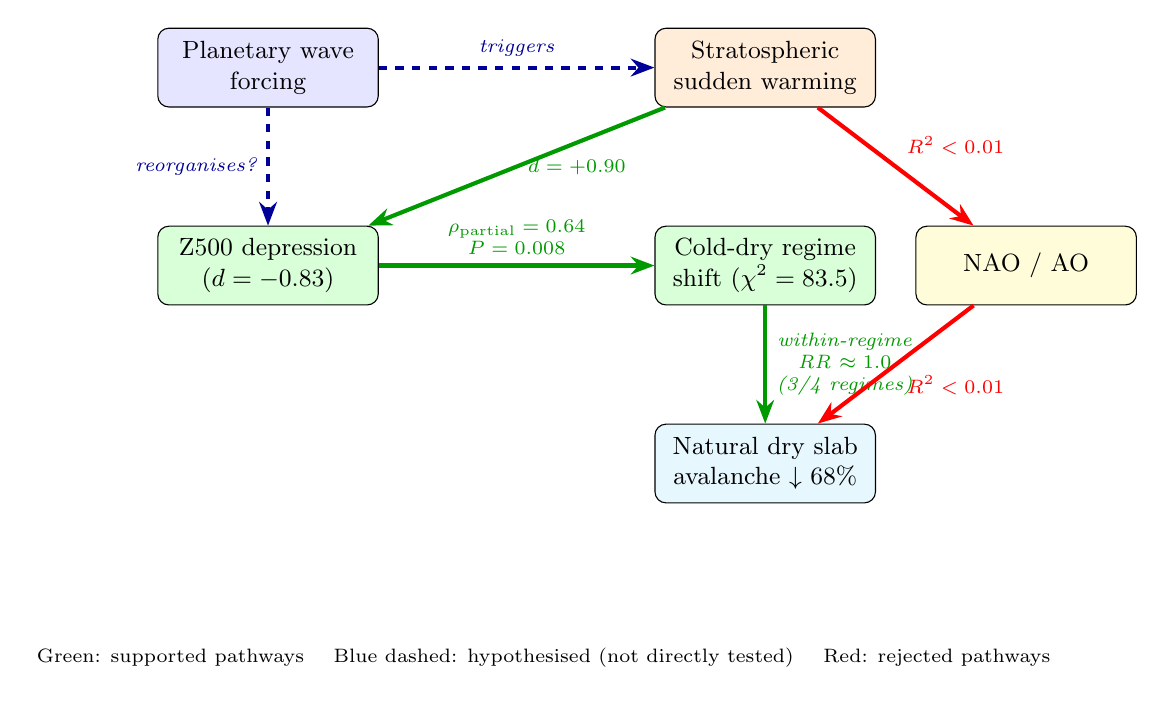
\begin{tikzpicture}[
    node distance=2.5cm and 3.5cm,
    every node/.style={draw, rounded corners, minimum width=2.8cm, minimum height=1cm, align=center, font=\small},
    arr/.style={-{Stealth[length=3mm]}, thick},
    xarr/.style={-{Stealth[length=3mm]}, thick, red, line width=1.5pt},
    garr/.style={-{Stealth[length=3mm]}, thick, green!60!black, line width=1.5pt},
    harr/.style={-{Stealth[length=3mm]}, thick, blue!60!black, line width=1.5pt, dashed},
]
% Nodes
\node (pw) [fill=blue!10] {Planetary wave\\forcing};
\node (ssw) [right=of pw, fill=orange!15] {Stratospheric\\sudden warming};
\node (nao) [below right=1.5cm and 0.5cm of ssw, fill=yellow!15] {NAO / AO};
\node (z500) [below=1.5cm of pw, fill=green!15] {Z500 depression\\($d = -0.83$)};
\node (regime) [right=of z500, fill=green!15] {Cold-dry regime\\shift ($\chi^2 = 83.5$)};
\node (aval) [below=1.5cm of regime, fill=cyan!10] {Natural dry slab\\avalanche $\downarrow$ 68\%};

% Supported pathway arrows (green) - tropospheric chain
\draw[garr] (ssw) -- node[draw=none,right,font=\scriptsize\itshape,minimum width=0pt,minimum height=0pt] {$d = +0.90$} (z500);
\draw[garr] (z500) -- node[draw=none,above,font=\scriptsize\itshape,minimum width=0pt,minimum height=0pt] {$\rho_{\mathrm{partial}} = 0.64$\\$P = 0.008$} (regime);
\draw[garr] (regime) -- node[draw=none,right,font=\scriptsize\itshape,minimum width=0pt,minimum height=0pt] {within-regime\\RR $\approx 1.0$\\(3/4 regimes)} (aval);

% Hypothesised common-cause pathway (dashed blue) - not directly tested
\draw[harr] (pw) -- node[draw=none,above,font=\scriptsize\itshape,minimum width=0pt,minimum height=0pt] {triggers} (ssw);
\draw[harr] (pw) -- node[draw=none,left,font=\scriptsize\itshape,minimum width=0pt,minimum height=0pt] {reorganises?} (z500);

% Rejected pathways (red)
\draw[xarr] (ssw) -- node[draw=none,above right,font=\scriptsize\bfseries,minimum width=0pt,minimum height=0pt,text=red] {$R^2 < 0.01$} (nao);
\draw[xarr] (nao) -- node[draw=none,below right,font=\scriptsize\bfseries,minimum width=0pt,minimum height=0pt,text=red] {$R^2 < 0.01$} (aval);

% Legend
\node[draw=none, minimum width=0pt, minimum height=0pt, font=\scriptsize] at (3.5, -7.5) {Green: supported pathways \quad Blue dashed: hypothesised (not directly tested) \quad Red: rejected pathways};
\end{tikzpicture}
\caption{\textbf{Conceptual diagram for the SSW--avalanche association.}
The \textbf{primary pathway} (green arrows): tropospheric circulation reorganisation through Z500 blocking produces a weather regime shift toward cold-dry conditions. Partial-correlation analysis indicates that Z500 carries the signal: $\rho = 0.64$ ($P = 0.008$) after controlling for stratospheric vortex deceleration, whereas stratospheric metrics show no residual effect ($\rho = -0.28$, $P = 0.29$). The \textbf{common driver} (dashed blue): enhanced planetary-wave forcing simultaneously triggers the SSW and reorganises tropospheric circulation\cite{Polvani2004}; pre-SSW Z500 anomalies already predict the eventual avalanche response ($\rho = 0.51$, $P = 0.045$). Composite propagation shows warming descends from 10~hPa (lag~0) to 100~hPa (lag~$+20$~d), maintaining stratosphere--troposphere coupling throughout. Within each regime, SSW and non-SSW days show near-identical avalanche rates ($\mathrm{RR}_{\mathrm{within}} = 0.98$--$1.16$ in three of four regimes; warm-dry residual $\mathrm{IRR} = 1.89$, $P = 0.013$, attributable to seasonal clustering). The \textbf{rejected pathways} (red arrows): annular modes are not supported as surface-coupling channels ($R^2 < 0.01$ for both AO and NAO).}
\label{fig:dag}
\end{figure}

\begin{figure}[!ht]
\centering
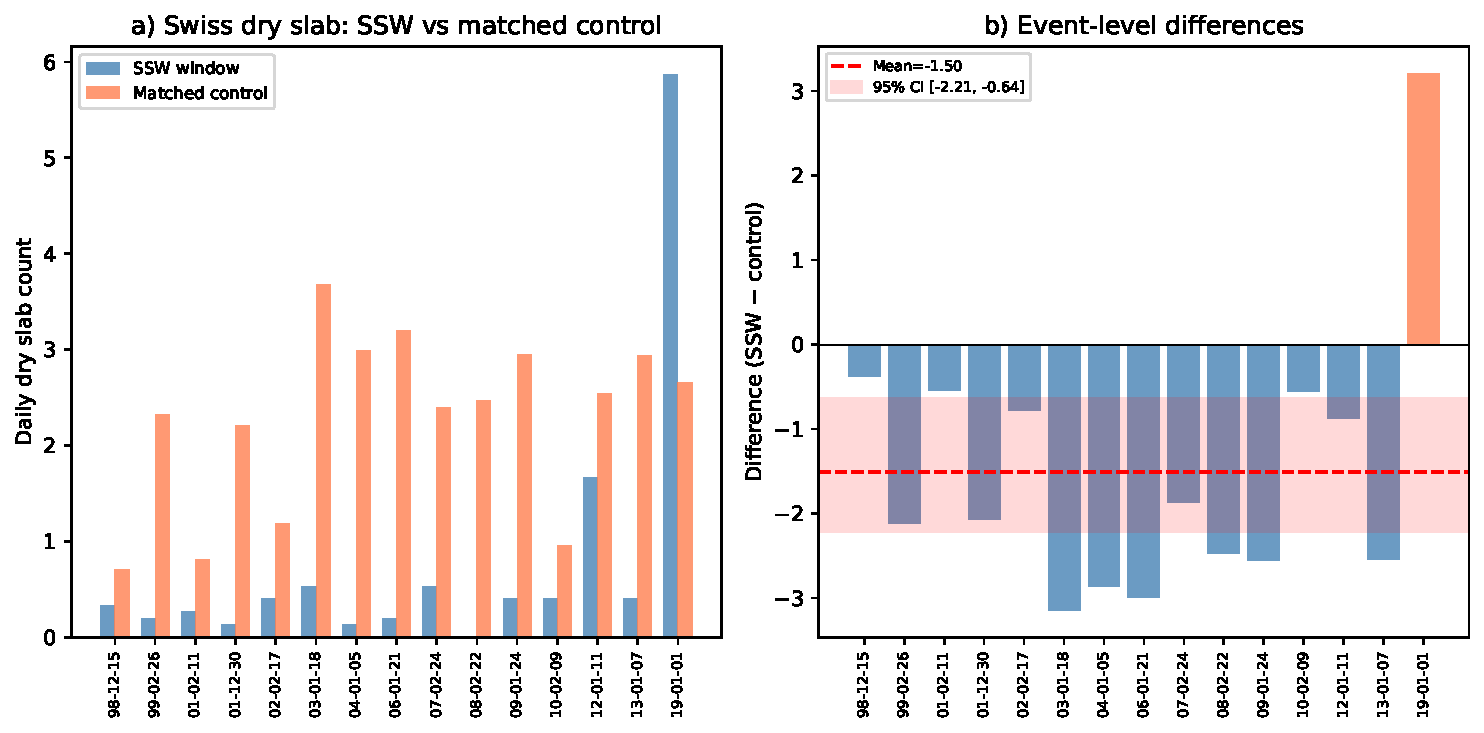
\includegraphics[width=\textwidth]{../data/figures/rev_fig1_ssw_swiss.pdf}
\caption{\textbf{SSW events suppress natural dry slab avalanche activity in Switzerland.}
\textbf{a},~Rate ratios (RR $=$ observed/expected) for 16~SSW events during 1998/99--2018/19, with expectation from day-of-year-matched non-SSW winters. Fourteen events have $\mathrm{RR} < 1$ and the geometric mean is 0.32; the only positive events are February~2018 ($\mathrm{RR} = 1.05$) and January~2019 ($\mathrm{RR} = 3.43$).
\textbf{b},~Winter-blocked bootstrap distribution of the geometric-mean RR (10,000 resamples). The 95\% CI $[0.26, 0.53]$ lies entirely below 1.0 (Supplementary Table~\ref{tab:winter_boot}).}
\label{fig:ssw_matched}
\end{figure}

\begin{figure}[!ht]
\centering
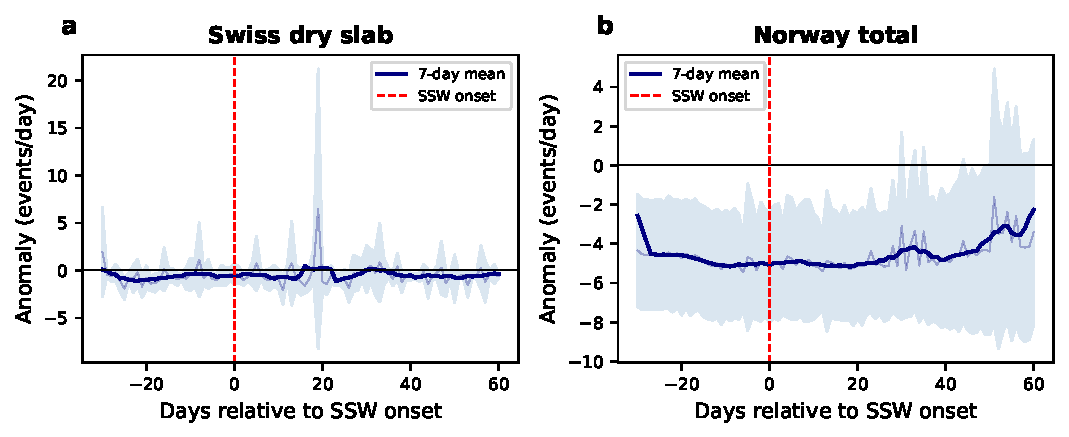
\includegraphics[width=\textwidth]{../data/figures/fig4_event_study_fresh.pdf}
\caption{\textbf{Event-study: daily avalanche anomalies around SSW onset.}
Composite anomalies (observed minus DOY-matched expectation) stacked across 16~SSW events, lags $-30$ to $+30$~days. Suppression begins about 13~days before onset and persists after onset; 13/16 events show pre-onset suppression during days $-15$ to $-6$ ($P = 0.011$). Blue shading: 95\% CI across events.}
\label{fig:event_study}
\end{figure}

\begin{figure}[!ht]
\centering
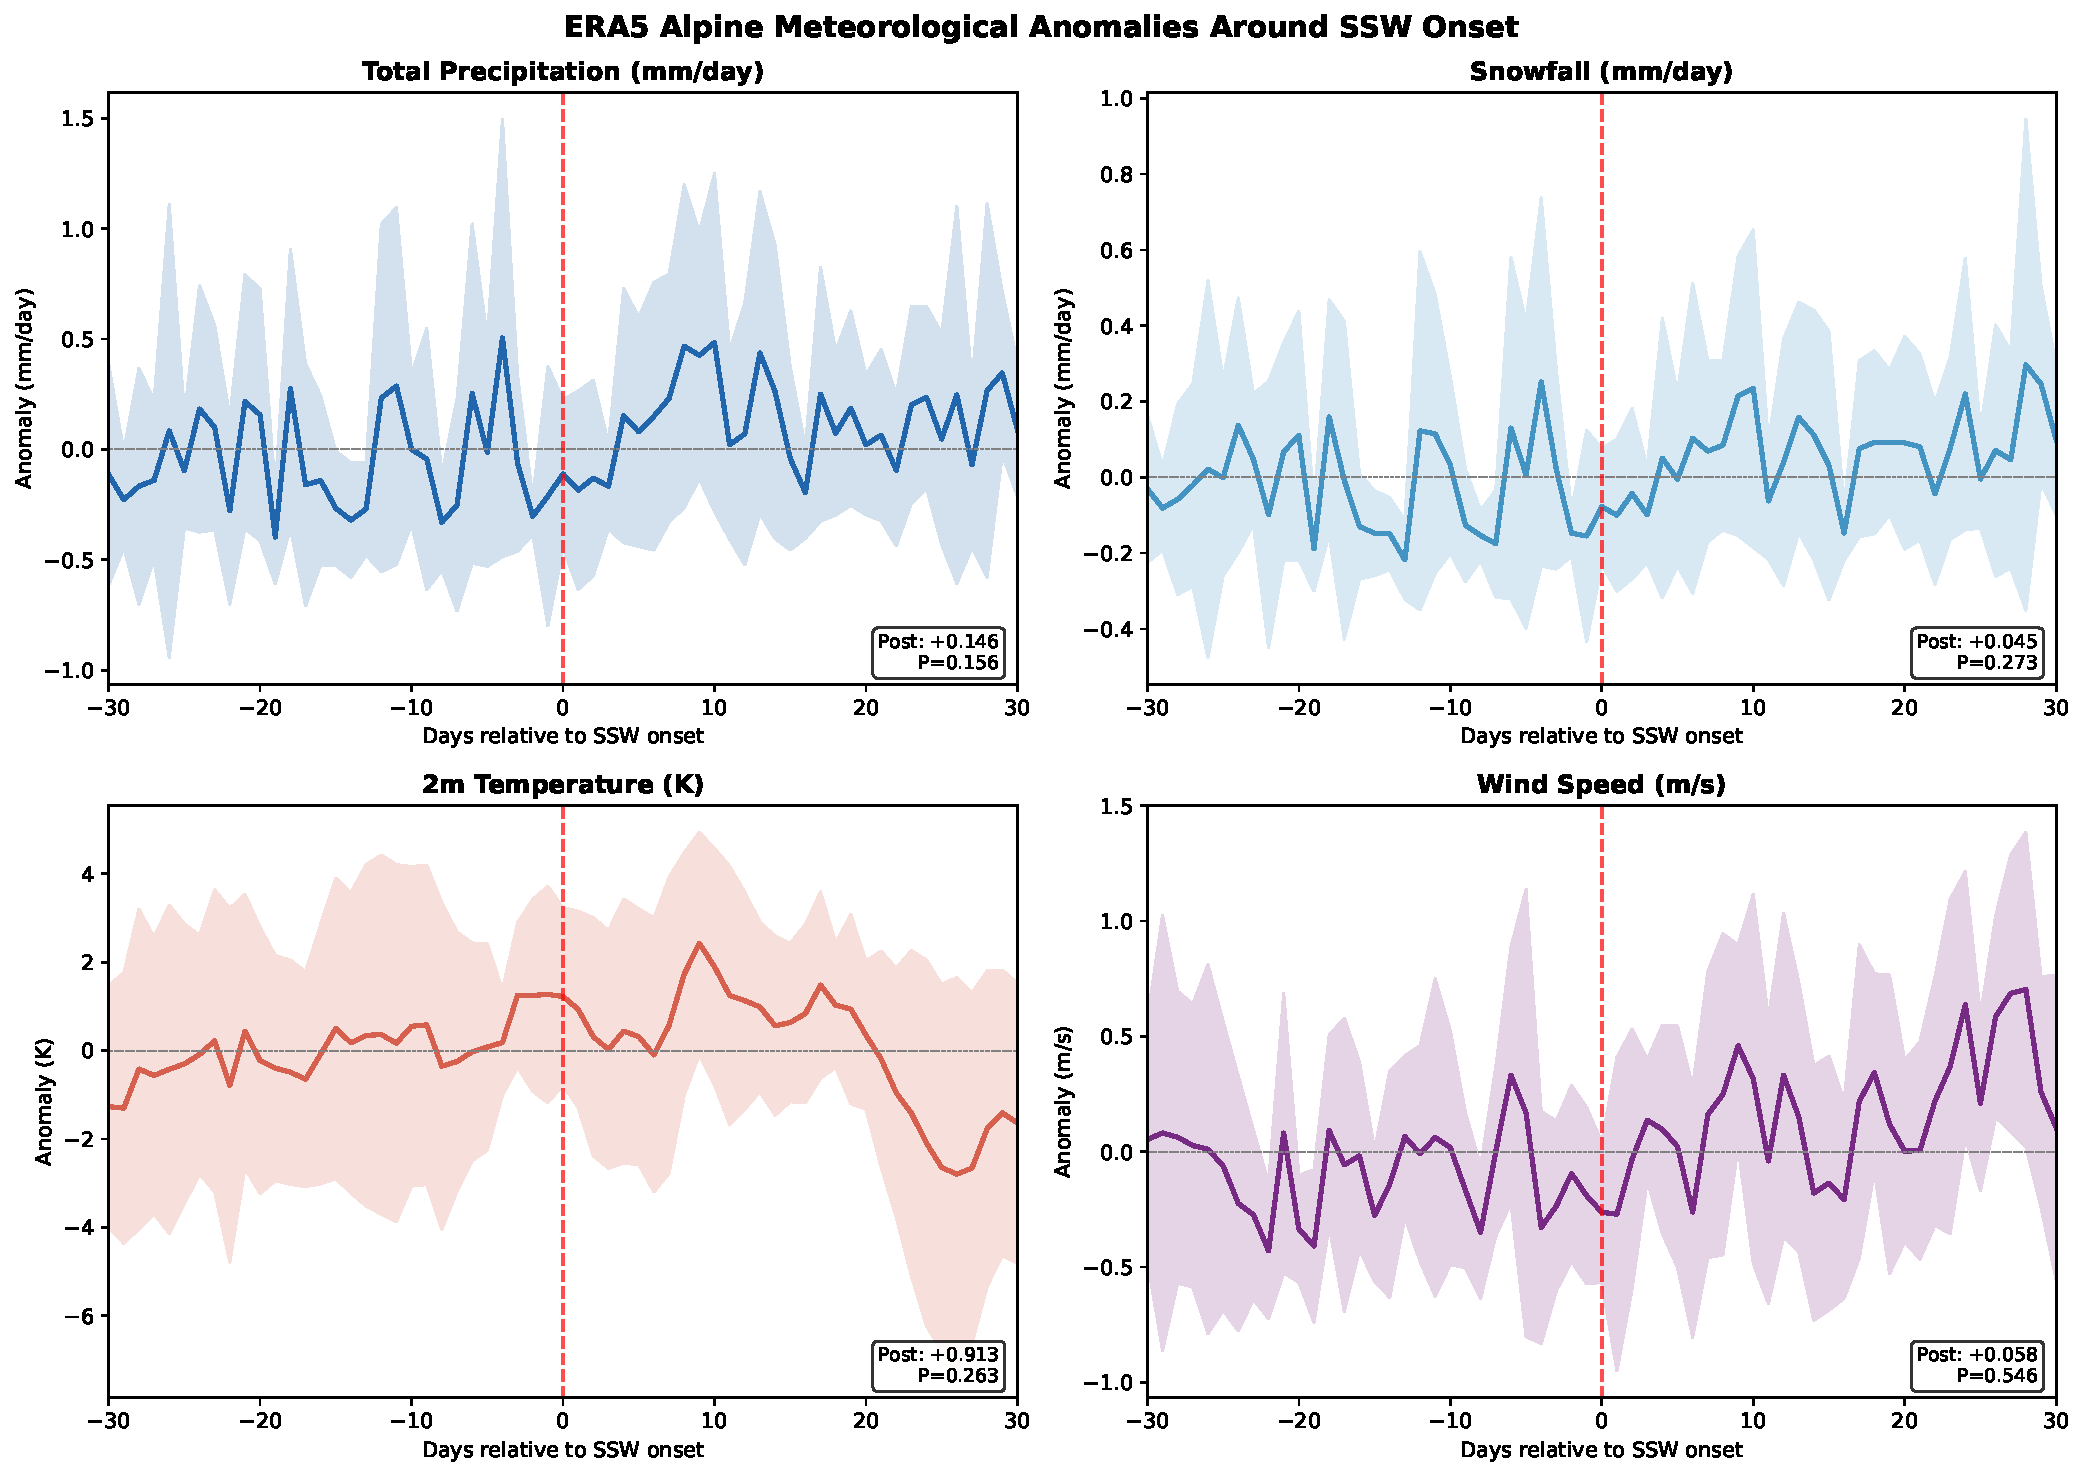
\includegraphics[width=\textwidth]{../data/figures/mech_fig1_era5_composites.pdf}
\caption{\textbf{ERA5 Alpine surface meteorology around SSW onset.}
Event-level composite anomalies for 16~SSW events (each event weighted equally).
\textbf{a},~2~m temperature: modest event-level cooling that does not reach significance ($\Delta T = -0.4$~K, $P = 0.32$, $n = 16$).
\textbf{b},~Snowfall: no change ($P > 0.99$).
\textbf{c},~Wind speed: no change.
Event-level temperature and precipitation explain only $\sim$1\% of the avalanche signal ($R^2 = 0.011$), indicating that synoptic-scale circulation reorganisation, not local surface meteorology, dominates event-level variability. Shaded bands: 95\% CI.}
\label{fig:era5_composites}
\end{figure}

\begin{figure}[!ht]
\centering
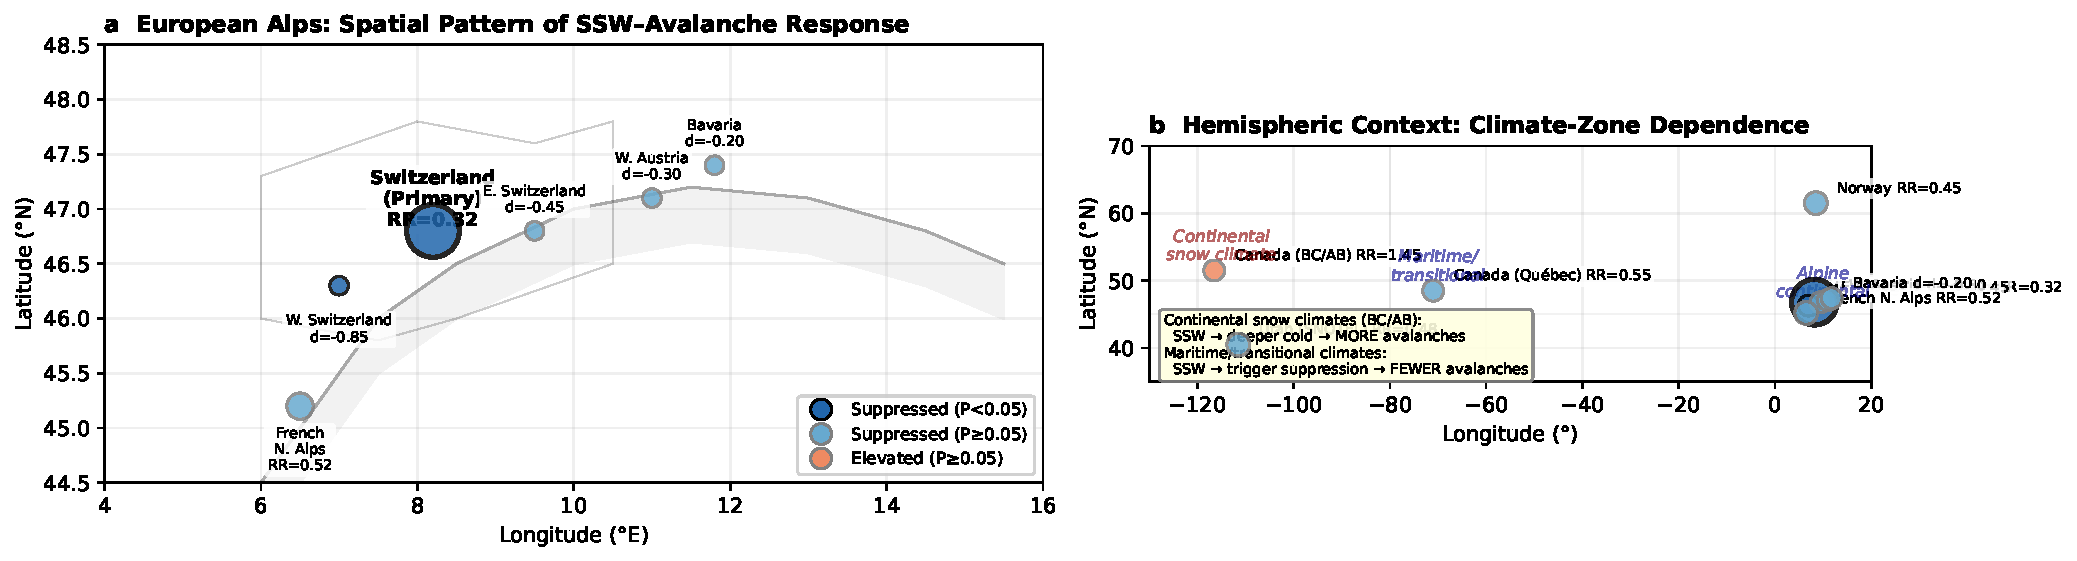
\includegraphics[width=\textwidth]{../data/figures/fig_geographic_effect_map.pdf}
\caption{\textbf{Geographic pattern of SSW--avalanche response across the Northern Hemisphere.}
\textbf{a},~European Alps detail using EAWS data from two SSW events ($n_{\mathrm{eff}} = 2$; hypothesis-generating only). Circle size scales with sample size and colour indicates effect direction.
\textbf{b},~Hemispheric context. Continental and transitional snow climates (Switzerland, Norway, Utah, Qu\'ebec) show suppression, whereas western Canadian ranges (BC/AB) show elevation, consistent with climate-zone-dependent response.}
\label{fig:geographic_map}
\end{figure}

\begin{figure}[!ht]
\centering
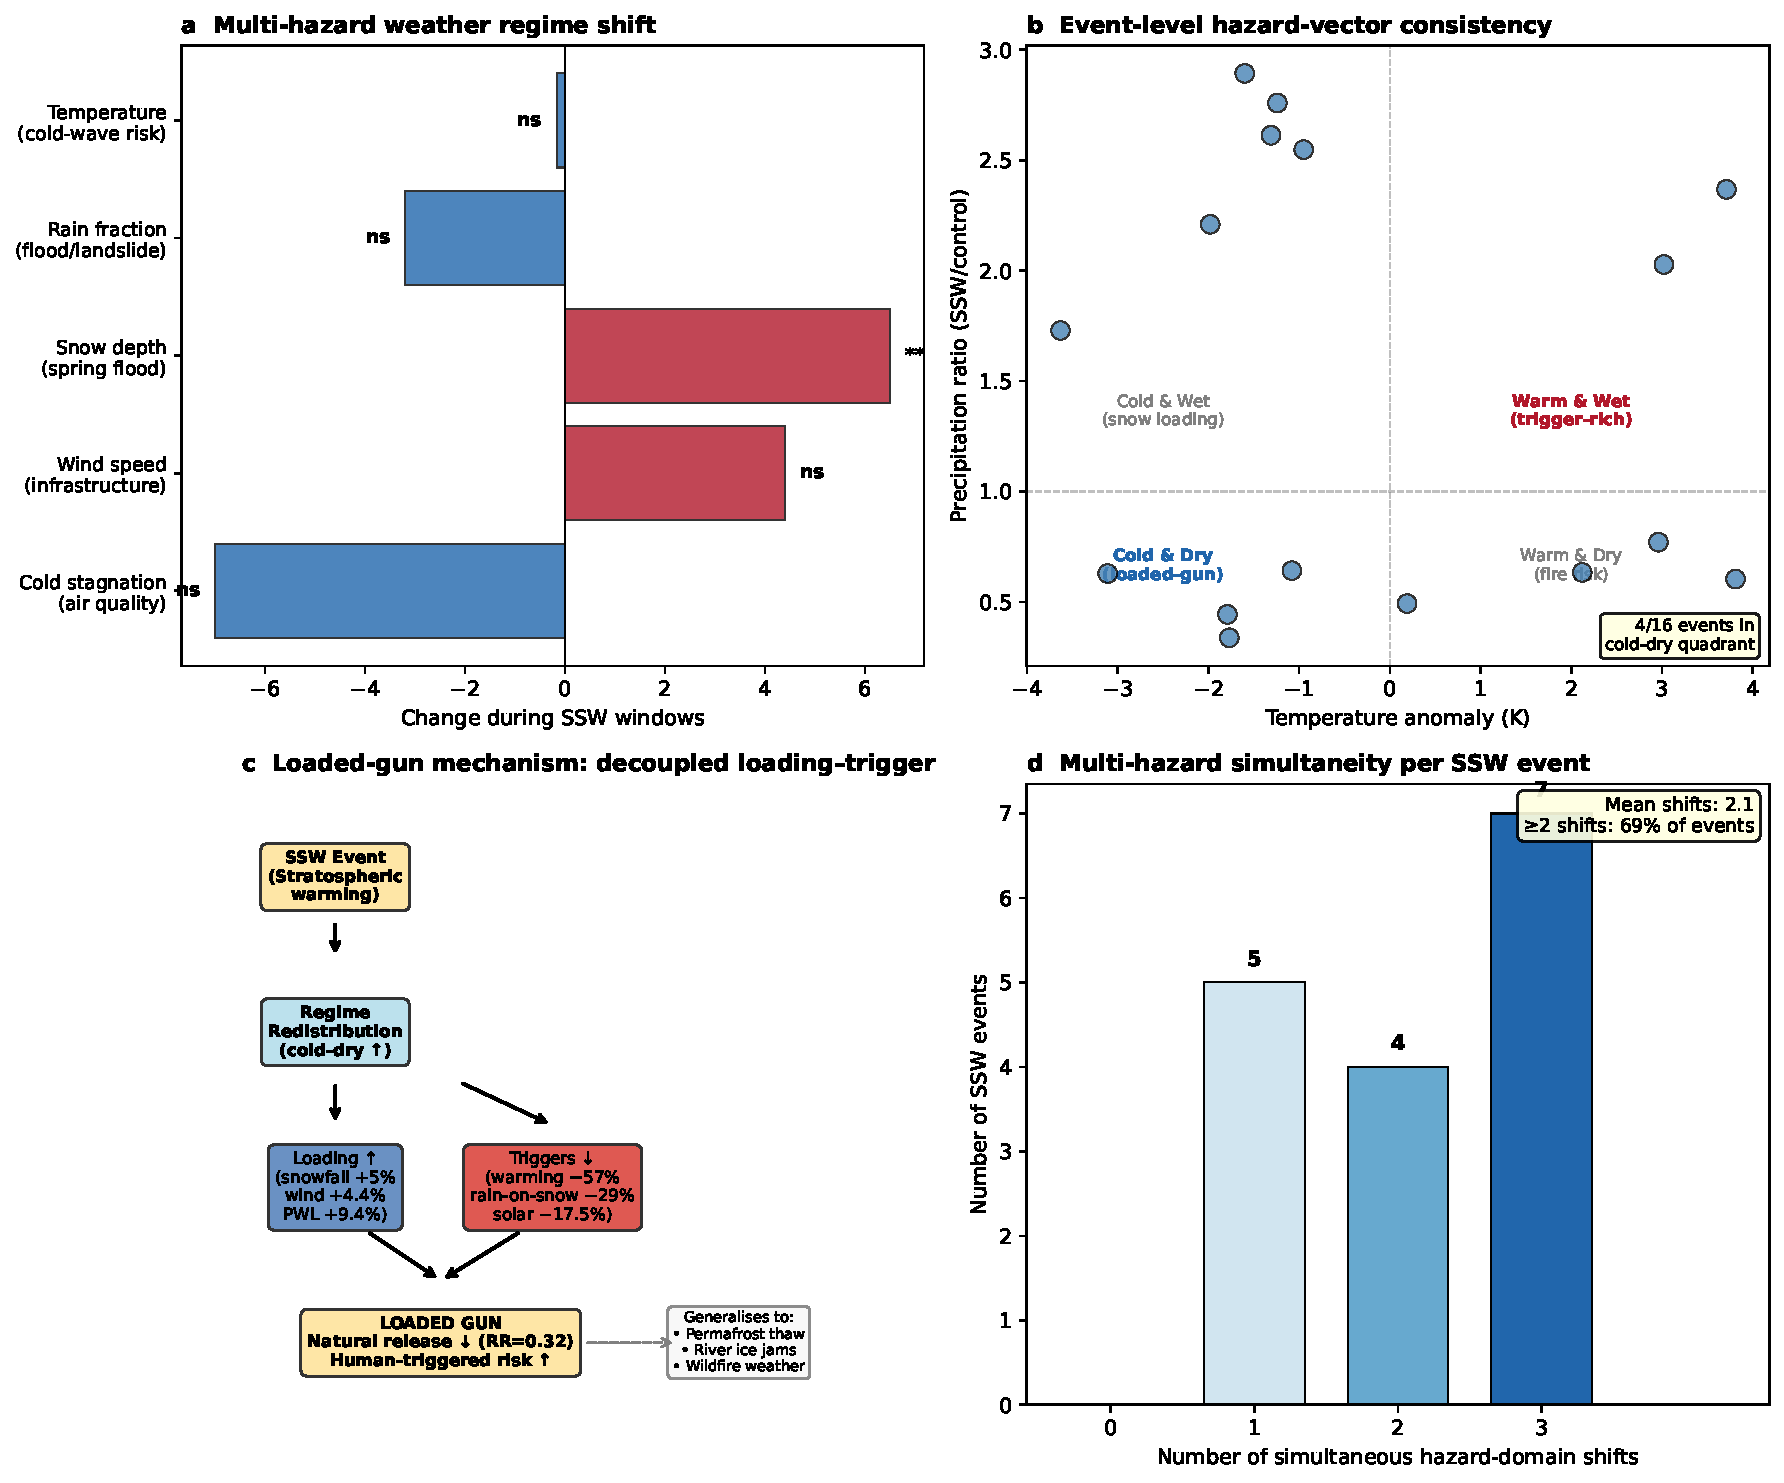
\includegraphics[width=\textwidth]{../data/figures/fig_multi_hazard_regime.pdf}
\caption{\textbf{SSW regime redistribution affects multiple hazard domains simultaneously.}
\textbf{a},~Weather shifts during SSW windows relative to DOY-matched controls. Snow depth and SWE increase, whereas temperature and rain fraction decrease, indicating loading with trigger suppression.
\textbf{b},~Event-level hazard-vector consistency: each SSW event plotted in temperature-anomaly versus precipitation-ratio space. Events cluster in the cold-dry quadrant, the loaded-gun regime.
\textbf{c},~Mechanistic schematic of how regime redistribution decouples loading from triggers to produce the loaded-gun state.
\textbf{d},~Multi-hazard simultaneity: 69\% of SSW events shift $\geq$2 hazard domains simultaneously (mean 2.1 domains per event).}
\label{fig:multi_hazard}
\end{figure}

\begin{figure}[!ht]
\centering
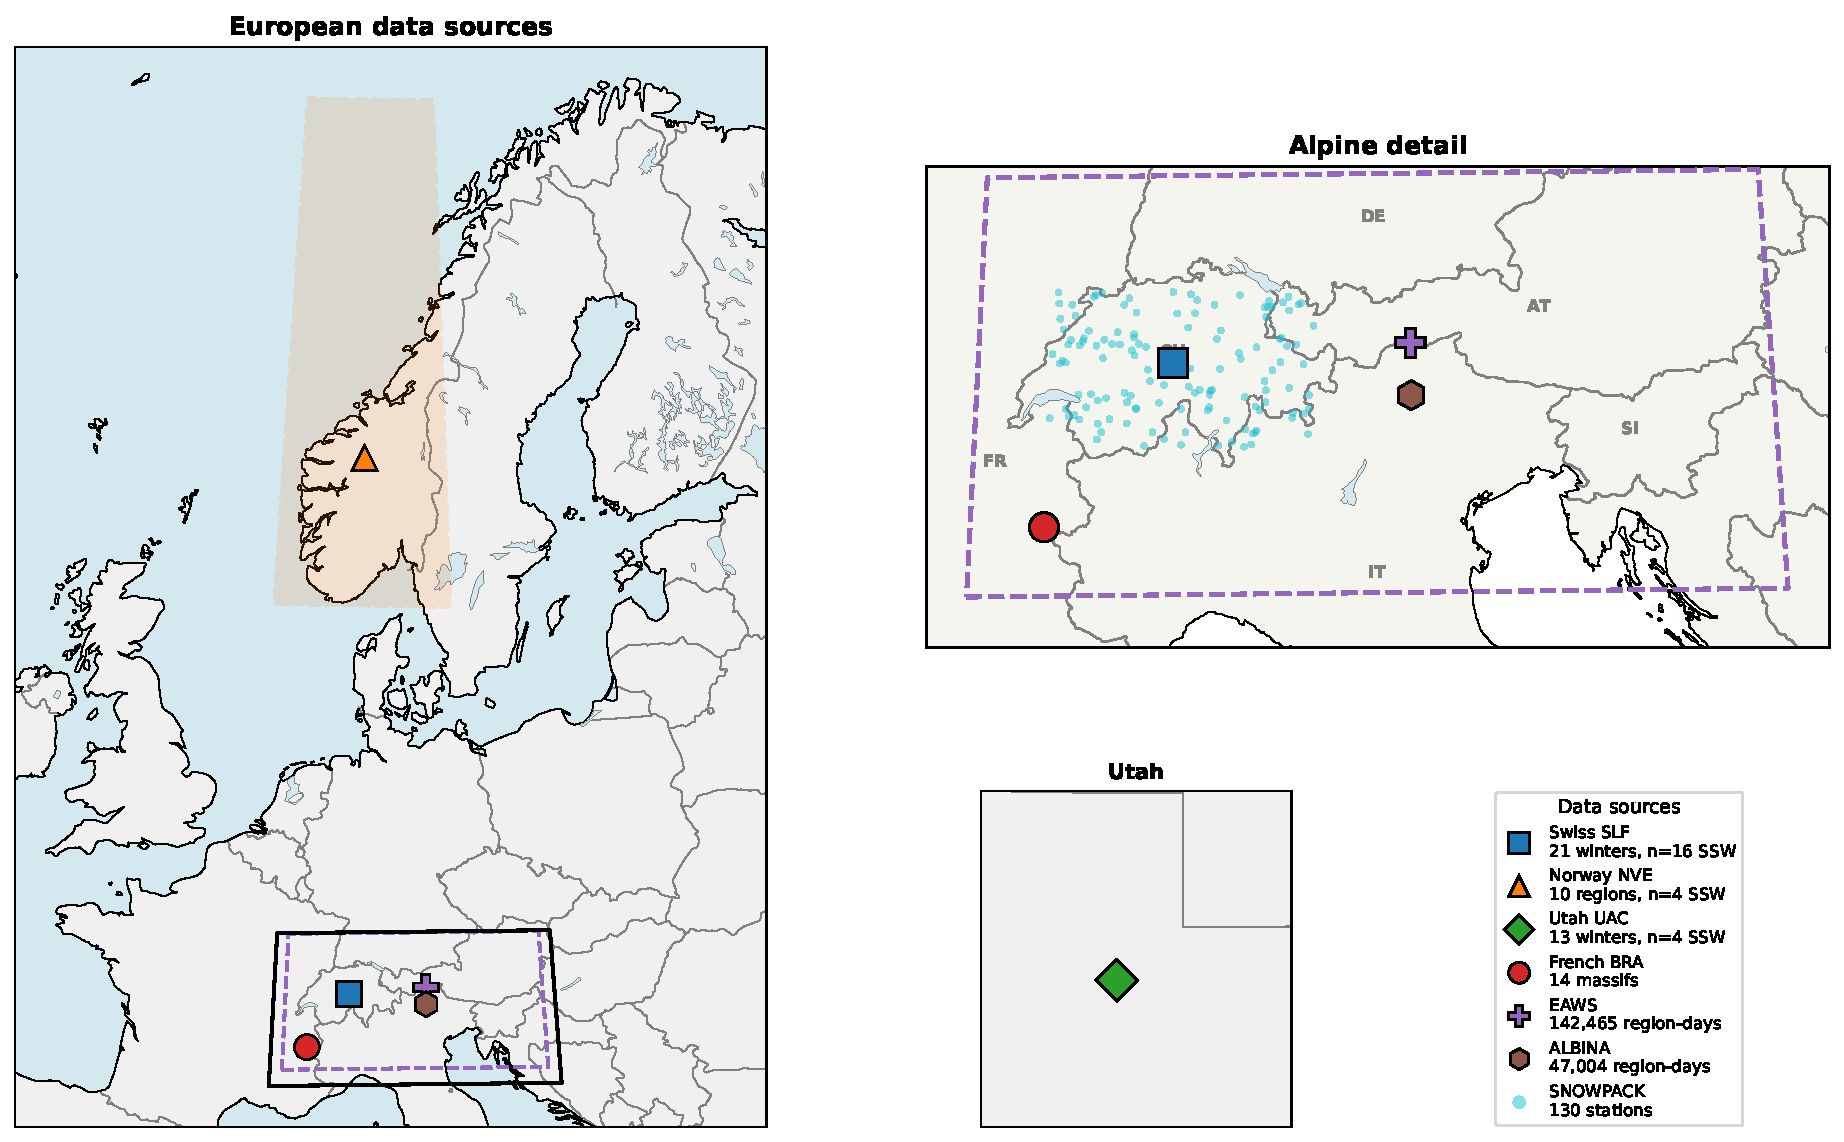
\includegraphics[width=\textwidth]{../data/figures/fig_study_area_map.pdf}
\caption{\textbf{Study area and data sources.}
\textbf{Left},~European overview showing primary (Switzerland, Norway) and validation (France, EAWS, ALBINA) datasets.
\textbf{Centre},~Alpine detail with the Swiss SLF domain, 130 SNOWPACK stations, French BRA massifs, and the EAWS/ALBINA network.
\textbf{Bottom right},~Utah Avalanche Center domain. Data spans are listed in Methods.}
\label{fig:study_area}
\end{figure}

\begin{figure}[!ht]
\centering
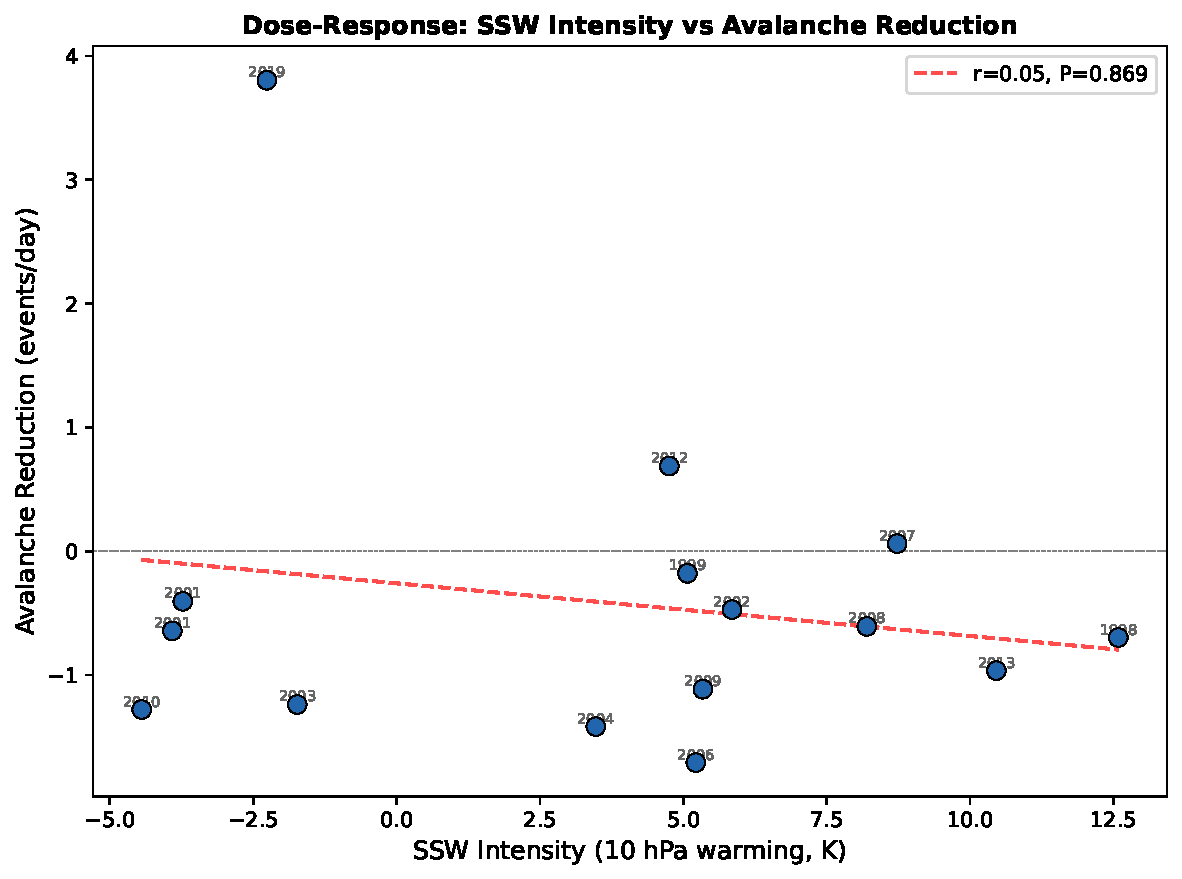
\includegraphics[width=\textwidth]{../data/figures/mech_fig5_dose_response.pdf}
\caption{\textbf{Wave-forcing proxy dose--response and direct $\overline{v'T'}$ validation.}
\textbf{a,}~Vortex-deceleration proxy versus event-level $\log(\mathrm{RR})$ ($\rho = -0.54$, $P = 0.032$; exploratory and not BH-FDR significant).
\textbf{b,}~Direct zonal-mean poleward eddy heat flux $\overline{v'T'}$ at 100~hPa versus $\log(\mathrm{RR})$ ($\rho = -0.25$, $P = 0.34$). The direct forcing metric is weaker, consistent with Alpine blocking being a better event-level carrier than stratospheric intensity alone.}
\label{fig:ep_flux_dose}
\end{figure}

\begin{figure}[!ht]
\centering
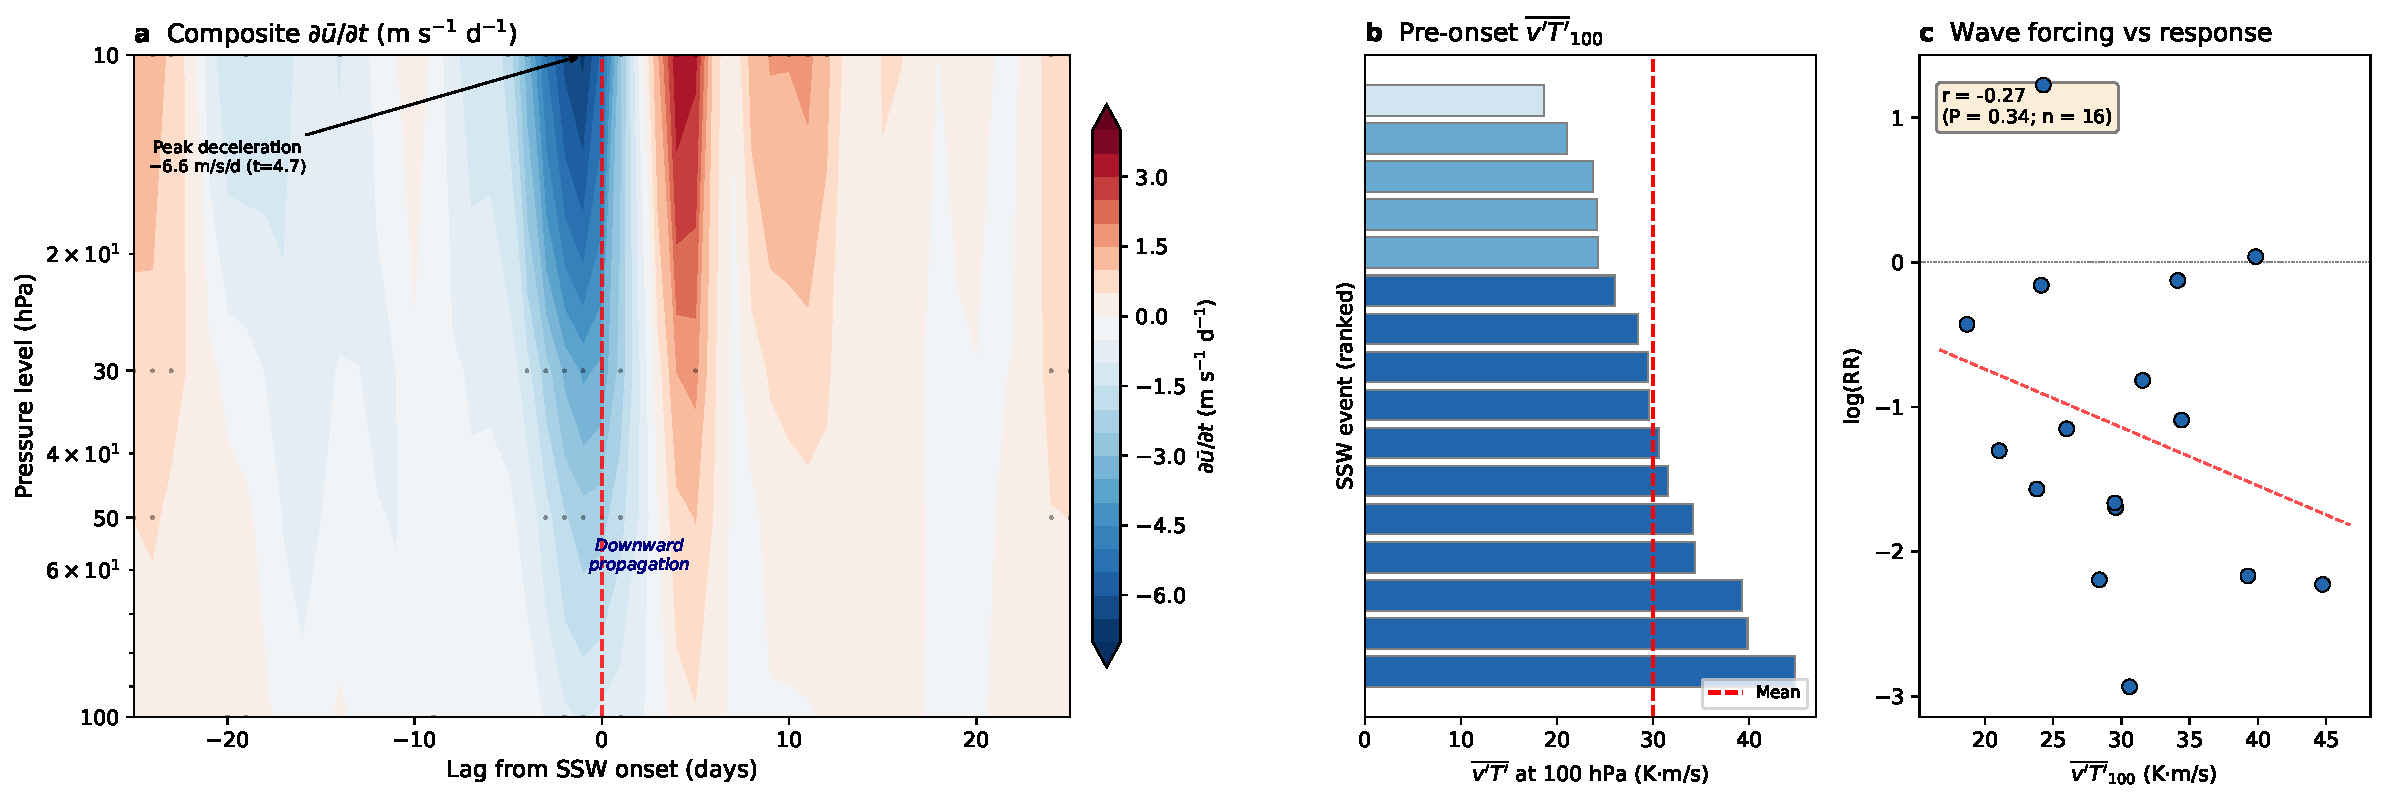
\includegraphics[width=\textwidth]{../data/figures/fig_epflux_height_time.pdf}
\caption{\textbf{Stratospheric wave-forcing composites for 16~SSW events.}
\textbf{a},~Height--time composite of zonal-wind tendency across four pressure levels. Peak deceleration reaches $-6.6$~m~s$^{-1}$~d$^{-1}$ at 10~hPa and descends to $-1.1$~m~s$^{-1}$~d$^{-1}$ at 100~hPa in about 6.6~days, consistent with published SSW composites\cite{Butler2017}.
\textbf{b},~Pre-onset $\overline{v'T'}$ at 100~hPa for each event. All 16 events show positive anomalies.
\textbf{c},~Event-level $\overline{v'T'}$ versus $\log(\mathrm{RR})$ ($r = -0.27$, $P = 0.34$), indicating that forcing intensity does not robustly predict hazard magnitude within the SSW sample.}
\label{fig:epflux_composite}
\end{figure}

\begin{figure}[!ht]
\centering
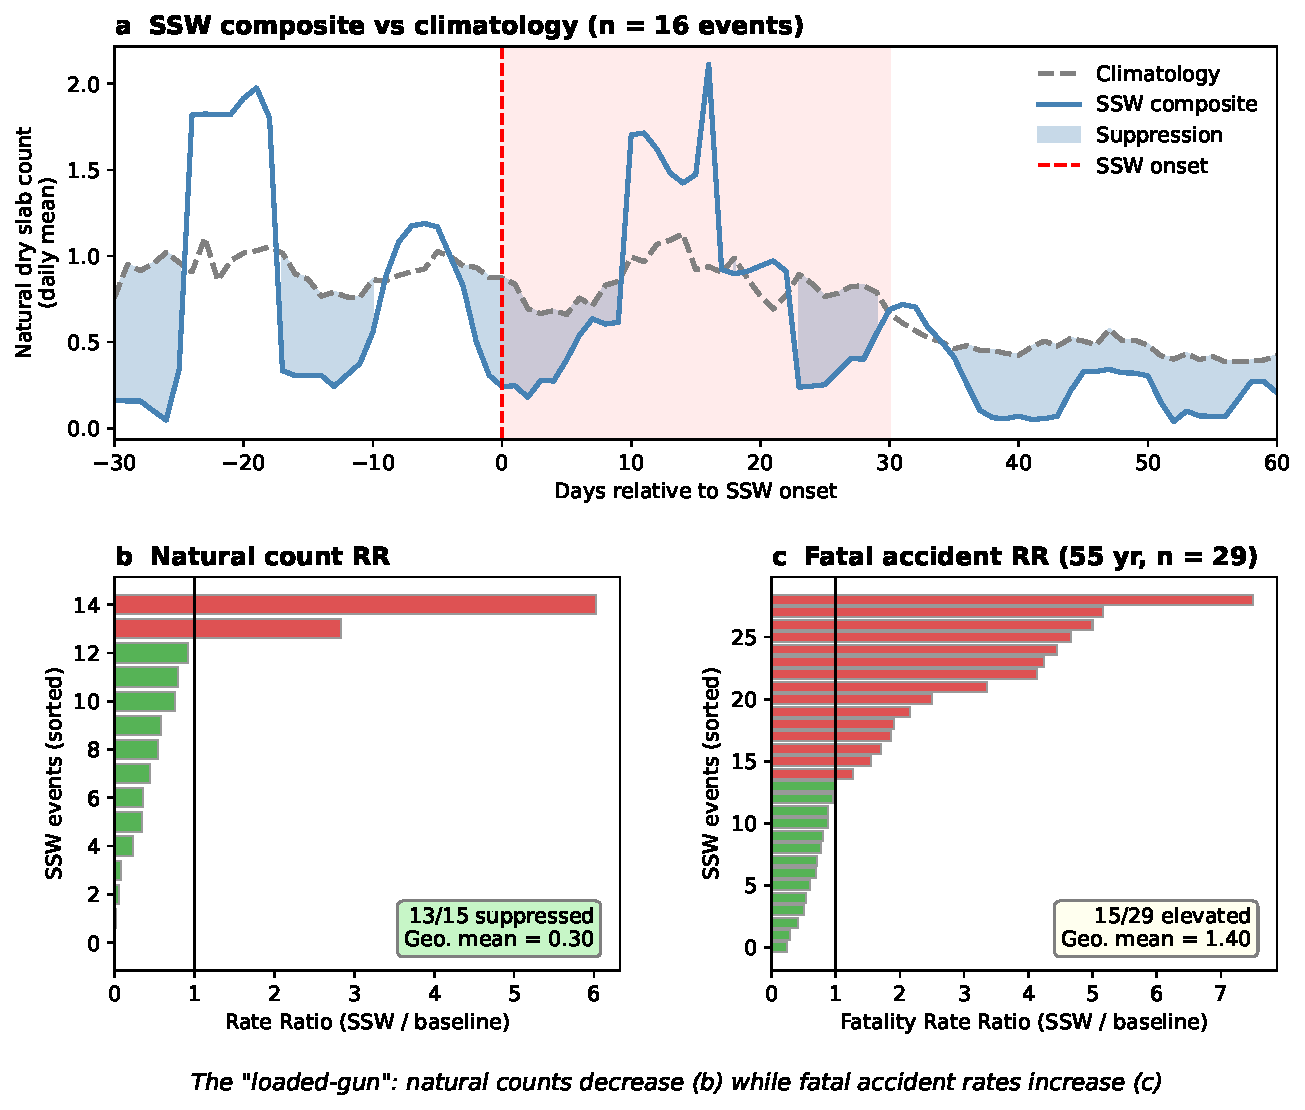
\includegraphics[width=\textwidth]{../data/figures/fig_count_rating_dissociation.pdf}
\caption{\textbf{The ``loaded-gun'' dissociation: natural trigger counts decrease while structural instability persists.}
\textbf{a,}~Composite natural dry slab activity for 16~SSW events versus DOY-matched non-SSW climatology. Natural activity remains suppressed through the post-onset window.
\textbf{b,}~Event-level natural-count rate ratios. Fourteen of 16 events have $\mathrm{RR} < 1$ and the geometric mean is 0.32.
\textbf{c,}~Event-level fatal-accident rate ratios over 55~years (29 events). The aggregate geometric mean is 1.40, but the event-level direction is mixed (15/29 above 1; permutation $P = 0.067$), providing supportive consequence-context only; the primary evidence for the loaded-gun state rests on the Swiss count suppression and SNOWPACK instability diagnostics.}
\label{fig:count_rating_dissociation}
\end{figure}

% ============================================================
%  EXTENDED DATA
% ============================================================
\clearpage
\section*{Extended Data}

\begin{table}[!ht]
\centering
\caption{\textbf{Extended Data Table 1: Leave-one-out cross-validation.}
Sign-test $P$-values and geometric mean RR after dropping each SSW event in turn. All 16 jackknife folds remain significant at $P < 0.004$, demonstrating that no single event drives the result.}
\label{tab:loo}
\small
\begin{tabular}{lccc}
\toprule
Event dropped & Excluded RR & Remaining sign $P$ & Remaining geom.\ RR \\
\midrule
1998-12-15 & 0.88 & 0.004 & 0.30 \\
1999-02-26 & 0.44 & 0.004 & 0.32 \\
2001-02-11 & 0.18 & 0.004 & 0.33 \\
2001-12-30 & 0.11 & 0.004 & 0.35 \\
2002-02-17 & 0.27 & 0.004 & 0.32 \\
2003-01-18 & 0.19 & 0.004 & 0.34 \\
2004-01-05 & 0.11 & 0.004 & 0.35 \\
2006-01-21 & 0.21 & 0.004 & 0.34 \\
2007-02-24 & 0.32 & 0.004 & 0.32 \\
2008-02-22 & 0.05 & 0.004 & 0.36 \\
2009-01-24 & 0.11 & 0.004 & 0.35 \\
2010-02-09 & 0.65 & 0.004 & 0.31 \\
2012-01-11 & 0.85 & 0.004 & 0.30 \\
2013-01-07 & 0.34 & 0.004 & 0.32 \\
2018-02-12 & 1.05 & $< 0.001$ & 0.30 \\
2019-01-01 & 3.43 & $< 0.001$ & 0.28 \\
\bottomrule
\end{tabular}
\end{table}

\begin{table}[!ht]
\centering
\caption{\textbf{Extended Data Table 2: Phase-resolved analysis.}
Rate ratios in four non-overlapping SSW lifecycle phases. All phases show suppression, with the strongest signal in the pre-SSW period---supporting a precursor wave-forced component rather than a purely post-onset pathway. Note: these four tests share the same 16 SSW events; phase-level $P$-values are included in the stratified BH-FDR correction (Supplementary Table~\ref{tab:fdr_stratified}), and within-event dependence may further inflate Type~I error.}
\label{tab:phases}
\small
\begin{tabular}{lcccc}
\toprule
Phase & Days relative to onset & $n$ decrease / total & Median RR & Sign $P$ \\
\midrule
Pre & $-15$ to $-6$ & 13/16 & 0.16 & 0.011 \\
Onset & $-5$ to $+5$ & 14/16 & 0.37 & 0.002 \\
Post & $+6$ to $+15$ & 12/16 & 0.22 & 0.038 \\
Late & $+16$ to $+30$ & 12/16 & 0.29 & 0.038 \\
\bottomrule
\end{tabular}
\end{table}

\begin{table}[!ht]
\centering
\caption{\textbf{Extended Data Table 3: Multi-country evidence summary.}
Concordance across three countries using independent measurement systems. The Swiss and Norwegian results use different instruments (occurrence counts vs.\ danger forecasts); however, Norway's four SSW events share only two independent event windows ($n_{\mathrm{eff}} = 2$), and all multi-country evidence shares the same SSW event timing.}
\label{tab:multi}
\small
\begin{tabular}{lcccccc}
\toprule
Country & Measure & $n$ events & $n$ decrease & Effect size & $P$ & Cohen's $d$ \\
\midrule
Switzerland & Natural dry slab count & 16 & 14 & $\mathrm{RR} = 0.32$ & 0.002 & $-1.06$ \\
Norway & NVE danger level & 4 & 4 & $\Delta = -0.48$ & $< 10^{-6}$\textsuperscript{$\dagger$} & $-0.67$ \\
Utah & Dry slab count & 4 & 4 & $\mathrm{RR} = 0.34$ & 0.063 & --- \\
\midrule
\multicolumn{2}{l}{Combined (22/24 event-level pairs)} & 24 & 22 & --- & $< 10^{-5}$ & --- \\
\bottomrule
\multicolumn{7}{l}{\textsuperscript{$\dagger$}\scriptsize Daily-level MW test; $n_{\mathrm{eff}} = 2$ independent events (pre-2013 data carry constant fill values).}
\end{tabular}
\end{table}

\begin{table}[!ht]
\centering
\caption{\textbf{Extended Data Table 4: Rutschblock stability class distribution.}
Stability class frequencies during SSW windows ($\pm$15~d) versus non-SSW periods. SSW windows show fewer unstable profiles (class~1) and more very stable profiles (class~4).}
\label{tab:rutsch}
\small
\begin{tabular}{lcccc}
\toprule
Stability class & SSW ($n = 961$) & Non-SSW ($n = 3{,}472$) & SSW \% & Non-SSW \% \\
\midrule
1 (least stable) & 342 & 1,413 & 35.6\% & 40.7\% \\
2 & 387 & 1,296 & 40.3\% & 37.3\% \\
3 & 128 & 458 & 13.3\% & 13.2\% \\
4 (most stable) & 104 & 305 & 10.8\% & 8.8\% \\
\midrule
\multicolumn{5}{l}{Mann--Whitney $P = 0.003$ (one-sided, SSW more stable); Cohen's $d = 0.10$} \\
\bottomrule
\end{tabular}
\end{table}

\begin{table}[!ht]
\centering
\caption{\textbf{Extended Data Table 4b: Persistent weak-layer depth validation.}
SNOWPACK penetration depth (Pen\_depth) and critical crack length (min\_ccl\_pen) at the most critical persistent weak layer during SSW windows ($\pm$15~d) versus controls, across 130 Swiss stations (winter months only). Station-day values are shown for process characterisation; event-level sign tests ($n = 16$) provide proper inferential statistics (Supplementary Table~\ref{tab:event_level_snowpack}).}
\label{tab:pwl_depth}
\small
\begin{tabular}{lccccc}
\toprule
Metric & SSW & Control & Cohen's $d$ & Events & Sign $P$ \\
\midrule
Pen\_depth mean (cm) & 20.5 & 18.0 & 0.31 & 15/16 & 0.0005 \\
Pen\_depth median (cm) & 19.0 & 17.1 & --- & --- & --- \\
Fraction in 0.2--1.2~m & 43.5\% & 34.5\% & --- & 12/16 & 0.077 \\
min\_ccl at Pen\_depth & 0.44 & 0.66 & $-0.32$ & 14/16 & 0.004 \\
PWL prevalence (top 1~m) & 77.4\% & 64.4\% & --- & 13/16 & 0.021 \\
Joint critical (sk38 $< 1.5$) & 29.7\% & 21.9\% & --- & --- & --- \\
Loaded-gun signature & 28.3\% & 22.7\% & --- & --- & --- \\
\midrule
\multicolumn{6}{l}{$n_{\mathrm{SSW}} = 38{,}742$; $n_{\mathrm{ctrl}} = 246{,}415$ station-days; event-level $n = 16$} \\
\multicolumn{6}{l}{Loaded-gun: naturally stable (sn38 $> 2.0$) + skier-triggerable (sk38 $< 1.5$) + PWL present} \\
\bottomrule
\end{tabular}
\end{table}

% AO/NAO independence results are presented in Extended Data Table 11 (synoptic circulation coupling)

\begin{table}[!ht]
\centering
\caption{\textbf{Extended Data Table 5: Utah event-level results.}
Rate ratios for each SSW event in the Utah Avalanche Center database (2012--2025). All four events show decreased dry slab activity, consistent with the Swiss pattern.}
\label{tab:utah}
\small
\begin{tabular}{lcccc}
\toprule
SSW event & Observed & Expected & RR & Direction \\
\midrule
2013-01-07 & 9 & 57.4 & 0.16 & Decrease \\
2018-02-12 & 23 & 50.0 & 0.46 & Decrease \\
2019-01-01 & 33 & 55.5 & 0.60 & Decrease \\
2021-01-05 & 17 & 57.6 & 0.30 & Decrease \\
\midrule
\multicolumn{3}{l}{Geometric mean RR: 0.34} & \multicolumn{2}{l}{Sign test $P = 0.063$} \\
\bottomrule
\end{tabular}
\end{table}

\begin{table}[!ht]
\centering
\caption{\textbf{Extended Data Table 6: Complete mechanism chain and pathway tests.}
Every link in the SSW $\to$ avalanche chain with effect sizes, significance, and interpretation. All links in the identified pathway are independently significant. The within-regime residual ($\mathrm{IRR} = 0.89$, $P = 0.06$) is consistent with regime redistribution as the primary surface-coupling pathway but does not reach significance; full vs partial regime absorption cannot be distinguished at this sample size. Rejected pathways (AO, NAO, sintering) are listed for completeness.}
\label{tab:mechanism}
\small
\begin{adjustbox}{max width=\textwidth}
\begin{tabular}{lccccl}
\toprule
Link / pathway & Variable & $d$ or statistic & $P$ & $R^2$ & Interpretation \\
\midrule
\multicolumn{6}{l}{\textit{Identified mechanism chain (all links $P < 0.05$)}} \\
1. Strat.\ warming & T(50~hPa) & $d = +0.90$ & $6 \times 10^{-57}$ & --- & By definition \\
2. Z500 depression & Z500 (NH) & $d = -0.83$ & $5 \times 10^{-74}$ & --- & Highly significant \\
3. Surface cooling & T2m (Alpine) & $d = -0.69$ & $< 10^{-47}$ & --- & Large shift \\
4. Precip reduction & Precip (Alpine) & $d = -0.12$ & 0.001 & --- & Moderate shift \\
5. Regime shift & $\chi^2 = 83.5$ & 4 regimes & $5 \times 10^{-18}$ & --- & Cold-dry doubled \\
6. Within-regime null & $\mathrm{RR}_\mathrm{w} \approx 1.0$ & 3/4 regimes n.s.\ & --- & --- & Regime-carried \\
\midrule
\multicolumn{6}{l}{\textit{Event-level predictors ($\log\mathrm{RR}$, $n = 16$ events)}} \\
Z500 (NH mean) & & $r = 0.56$ & 0.024 & 0.316 & Best single predictor \\
SLP (NH mean) & & $r = 0.52$ & 0.037 & 0.290 & Synoptic-scale \\
Surface only (T2m + precip) & & $r < 0.1$ & $> 0.7$ & 0.011 & Near zero \\
Z500 + surface & & $\Delta R^2$ & --- & 0.317 & Surface adds 0.001 \\
\midrule
\multicolumn{6}{l}{\textit{Confirmed supplementary evidence}} \\
Rutschblock stability & $\Delta = +0.09$ & $d = 0.10$ & 0.003 & --- & Modest field-stability increase \\
Dose--response (SLP) & Strong reorg. & $\mathrm{RR} = 0.19$ & --- & --- & vs.\ weak RR $= 0.56$ \\
\midrule
\multicolumn{6}{l}{\textit{Rejected pathways}} \\
AO coupling & & $r = -0.07$ & 0.79 & 0.005 & Rejected \\
NAO coupling & & $r = 0.03$ & 0.92 & $< 0.001$ & Rejected \\
Sintering (Arrhenius) & & 17\% slower & --- & --- & Consistent (cold $\to$ slow) \\
\bottomrule
\end{tabular}
\end{adjustbox}
\end{table}

\begin{table}[!ht]
\centering
\caption{\textbf{Extended Data Table 7: Benjamini--Hochberg FDR correction (main-text subset).}
Primary hypothesis tests ordered by raw $P$-value with FDR-corrected values. The stratified correction (Supplementary Table~\ref{tab:fdr_stratified}) is the primary method; the 29-test single-family table (Supplementary Table~7) is provided for comparison only.}
\label{tab:fdr}
\small
\begin{tabular}{lccl}
\toprule
Test & Raw $P$ & FDR $P$ & Status \\
\midrule
Norway MW (SSW vs.\ control) & $< 10^{-15}$ & $< 10^{-14}$ & Significant\textsuperscript{$\dagger$} \\
Combined sign (32/36) & $< 10^{-6}$ & $< 10^{-5}$ & Significant \\
Swiss permutation (10,000) & 0.0005 & 0.003 & Significant \\
Swiss Wilcoxon ($\log$RR) & $< 0.001$ & 0.003 & Significant \\
Swiss $t$-test ($\log$RR) & $< 0.001$ & 0.003 & Significant \\
Swiss sign test (14/16) & 0.002 & 0.006 & Significant \\
Norway pairs sign (14/16) & 0.002 & 0.006 & Significant \\
Rutschblock MW (1-sided) & 0.003 & 0.008 & Significant \\
Phase: onset (14/16) & 0.002 & 0.006 & Significant \\
Phase: pre-SSW (13/16, sign) & 0.011 & 0.024 & Significant \\
Phase: post (12/16) & 0.038 & 0.066 & Marginal \\
Phase: late (12/16) & 0.038 & 0.066 & Marginal \\
Utah sign (4/4) & 0.063 & 0.097 & Not sig. \\
ERA5 T2m (event-level) & 0.32 & 0.46 & Not sig. \\
AO coupling & 0.79 & 0.90 & Not sig. \\
Sintering model & 0.86 & 0.92 & Not sig. \\
NAO coupling & 0.92 & 0.92 & Not sig. \\
ERA5 snowfall & $> 0.99$ & $> 0.99$ & Not sig. \\
\bottomrule
\multicolumn{4}{l}{\textsuperscript{$\dagger$}\scriptsize Daily-level test; pre-2013 Norwegian data carry constant fill values ($n_{\mathrm{eff}} = 2$ post-2013 events).}
\end{tabular}
\end{table}

\begin{table}[!ht]
\centering
\caption{\textbf{Extended Data Table 8: Robustness and sensitivity.}
Combined results for SSW-type stratification and sensitivity to analytical choices. The result is insensitive to SSW type, DOY matching bandwidth, window width, and SSW definition. $P$ values here are sign-test (binomial) probabilities; corresponding one-sample $t$-test results on log(RR) are reported in the Supplementary Information.}
\label{tab:sensitivity}
\small
\begin{tabular}{lccc}
\toprule
Parameter & Geo.\ mean RR & $n$ decrease / 16 & Sign $P$ \\
\midrule
\multicolumn{4}{l}{\textit{SSW type (displacement vs.\ split-vortex; MW type difference $P = 1.00$)}} \\
Displacement ($n = 11$) & 0.33 & 10/11 & 0.006 \\
Split ($n = 5$) & 0.32 & 4/5 & 0.188 \\
Stricter definition ($> -5$~m/s; $n = 14$) & 0.33 & 12/14 & 0.006 \\
\midrule
\multicolumn{4}{l}{\textit{DOY matching bandwidth (window $= \pm$15~d)}} \\
$\pm$1 day & 0.33 & 14/16 & 0.002 \\
$\pm$2 days & 0.32 & 14/16 & 0.002 \\
$\pm$3 days (primary) & 0.32 & 14/16 & 0.002 \\
$\pm$5 days & 0.33 & 14/16 & 0.002 \\
$\pm$7 days & 0.33 & 14/16 & 0.002 \\
$\pm$10 days & 0.32 & 14/16 & 0.002 \\
\midrule
\multicolumn{4}{l}{\textit{SSW window width (DOY margin $= \pm$3~d)}} \\
$\pm$5 days & 0.38 & 12/16 & 0.038 \\
$\pm$7 days & 0.39 & 14/16 & 0.002 \\
$\pm$10 days & 0.34 & 12/16 & 0.038 \\
$\pm$12 days & 0.30 & 13/16 & 0.011 \\
$\pm$15 days (primary) & 0.32 & 14/16 & 0.002 \\
$\pm$20 days & 0.35 & 13/16 & 0.011 \\
$\pm$25 days & 0.31 & 13/16 & 0.011 \\
$\pm$30 days & 0.32 & 13/16 & 0.011 \\
\bottomrule
\end{tabular}
\end{table}

\begin{table}[!ht]
\centering
\caption{\textbf{Extended Data Table 9: Synoptic-scale circulation coupling.}
Correlations between hemispheric circulation anomalies and event-level avalanche response ($\log\mathrm{RR}$). Z500 explains 31\% of variance; adding surface weather contributes $< 0.1\%$ additional variance. Event-level surface weather correlations are near zero despite significant aggregate differences ($P < 0.001$).}
\label{tab:synoptic}
\small
\begin{tabular}{lccccc}
\toprule
Variable & Pearson $r$ & $P$ & $R^2$ & Scale & Aggregate $d$ \\
\midrule
\multicolumn{6}{l}{\textit{Synoptic-scale (significant event-level predictors)}} \\
NCEP Z500 (NH mean) & 0.56 & 0.024 & 0.31 & Hemispheric & $-0.83$ \\
NCEP SLP (NH mean) & 0.52 & 0.037 & 0.27 & Hemispheric & --- \\
NCEP U850 (NH mean) & $-0.32$ & 0.229 & 0.10 & Hemispheric & --- \\
\midrule
\multicolumn{6}{l}{\textit{Local surface (aggregate significant, event-level null)}} \\
ERA5 T2m (Alpine) & 0.04 & 0.90 & $< 0.01$ & Regional & $-0.69^{***}$ \\
ERA5 precip (Alpine) & $-0.10$ & 0.72 & 0.01 & Regional & $-0.12^{**}$ \\
ERA5 wind speed (Alpine) & 0.14 & 0.61 & 0.02 & Regional & 0.04 \\
\midrule
\multicolumn{6}{l}{\textit{Stratospheric (non-significant)}} \\
NCEP T 50~hPa & $-0.11$ & 0.70 & 0.01 & Stratospheric & $+0.90^{***}$ \\
NCEP U 50~hPa & $-0.10$ & 0.70 & 0.01 & Stratospheric & --- \\
\midrule
\multicolumn{6}{l}{\textit{Annular modes (non-significant)}} \\
AO index & $-0.07$ & 0.790 & $< 0.01$ & Hemispheric & --- \\
NAO index & 0.03 & 0.920 & $< 0.01$ & Atlantic & --- \\
\midrule
\multicolumn{6}{l}{\textit{Stepwise model comparison}} \\
\multicolumn{3}{l}{Z500 only} & 0.316 & \multicolumn{2}{l}{Best single predictor} \\
\multicolumn{3}{l}{Surface only (T2m + precip)} & 0.011 & \multicolumn{2}{l}{Near zero} \\
\multicolumn{3}{l}{Z500 + surface} & 0.317 & \multicolumn{2}{l}{$\Delta R^2 = 0.001$} \\
\bottomrule
\end{tabular}
\end{table}

\begin{table}[!ht]
\centering
\caption{\textbf{Extended Data Table 10: Outlier and robustness diagnostics.}
Grubbs test, robust statistics, and leave-one-out hindcast cross-validation results.}
\label{tab:outlier}
\small
\begin{tabular}{lcc}
\toprule
Diagnostic & Value & Interpretation \\
\midrule
\multicolumn{3}{l}{\textit{Grubbs outlier test (Jan 2019, RR $= 3.43$)}} \\
Grubbs $G$ statistic & 2.29 & Not significant \\
Critical value ($\alpha = 0.05$) & 2.59 & $G < G_{\mathrm{crit}}$ \\
\midrule
\multicolumn{3}{l}{\textit{Robust statistics}} \\
Median RR (all 16 events) & 0.31 & Insensitive to outlier \\
Without Jan 2019 ($n = 15$) & $\mathrm{RR} = 0.28$ & Stronger without outlier \\
$t$-test without Jan 2019 & $P < 0.0001$ & Highly significant \\
\midrule
\multicolumn{3}{l}{\textit{Hindcast cross-validation (LOO)}} \\
Direction accuracy & 14/16 (87.5\%) & $P = 0.002$ vs.\ chance \\
LOO Brier score & 0.213 & Raw LOO Brier score \\
Climatological Brier score & 0.109 & Base rate $p = 14/16 = 0.875$ \\
Brier skill score (1 $-$ BS/BS$_{\mathrm{clim}}$) & $-0.95$ & No skill vs.\ climatology$^{\dagger}$ \\
\midrule
\multicolumn{3}{l}{\textit{Power analysis}} \\
Min.\ detectable $d$ ($n = 16$, 80\% power) & 0.75 & ERA5 underpowered ($d \approx 0.2$) \\
\bottomrule
\multicolumn{3}{l}{\footnotesize $^{\dagger}$BSS $= 1 - 0.213/0.109 = -0.95$: LOO probabilities perform worse than} \\
\multicolumn{3}{l}{\footnotesize always predicting the climatological suppression rate. Direction accuracy is} \\
\multicolumn{3}{l}{\footnotesize high (87.5\%) but calibrated probability adds no value over the base rate.} \\
\end{tabular}
\end{table}

\begin{table}[!ht]
\centering
\caption{\textbf{Extended Data Table 11: Human-triggered avalanche response during SSW windows.}
Differential trigger response separating the all-type human-triggered signal from the type-specific dry slab signal. The divergence between natural and human triggers is consistent with wind-slab formation enhancing human-triggerable instability while cold-dry conditions suppress spontaneous release.}
\label{tab:human}
\small
\begin{tabular}{lcccl}
\toprule
Trigger--type combination & RR & $P$ & Direction & Interpretation \\
\midrule
Natural dry slab & 0.32 & 0.002 & Decrease & Primary signal \\
Human dry slab & 0.68 & 0.126 & Decrease (n.s.) & Weaker suppression \\
Human all types & 1.45 & --- & Increase & Wind-slab dominated \\
Human/natural ratio shift & $1.81\times$ & 0.058 & Shift to human & Differential response \\
\midrule
Austrian LAWIS incidents & Increase & --- & Increase & Consistent (human-dominated) \\
\bottomrule
\end{tabular}
\end{table}

% EAWS geographic gradient figure moved to Supplementary Information (n_eff = 2 events)

\begin{figure}[!ht]
\centering
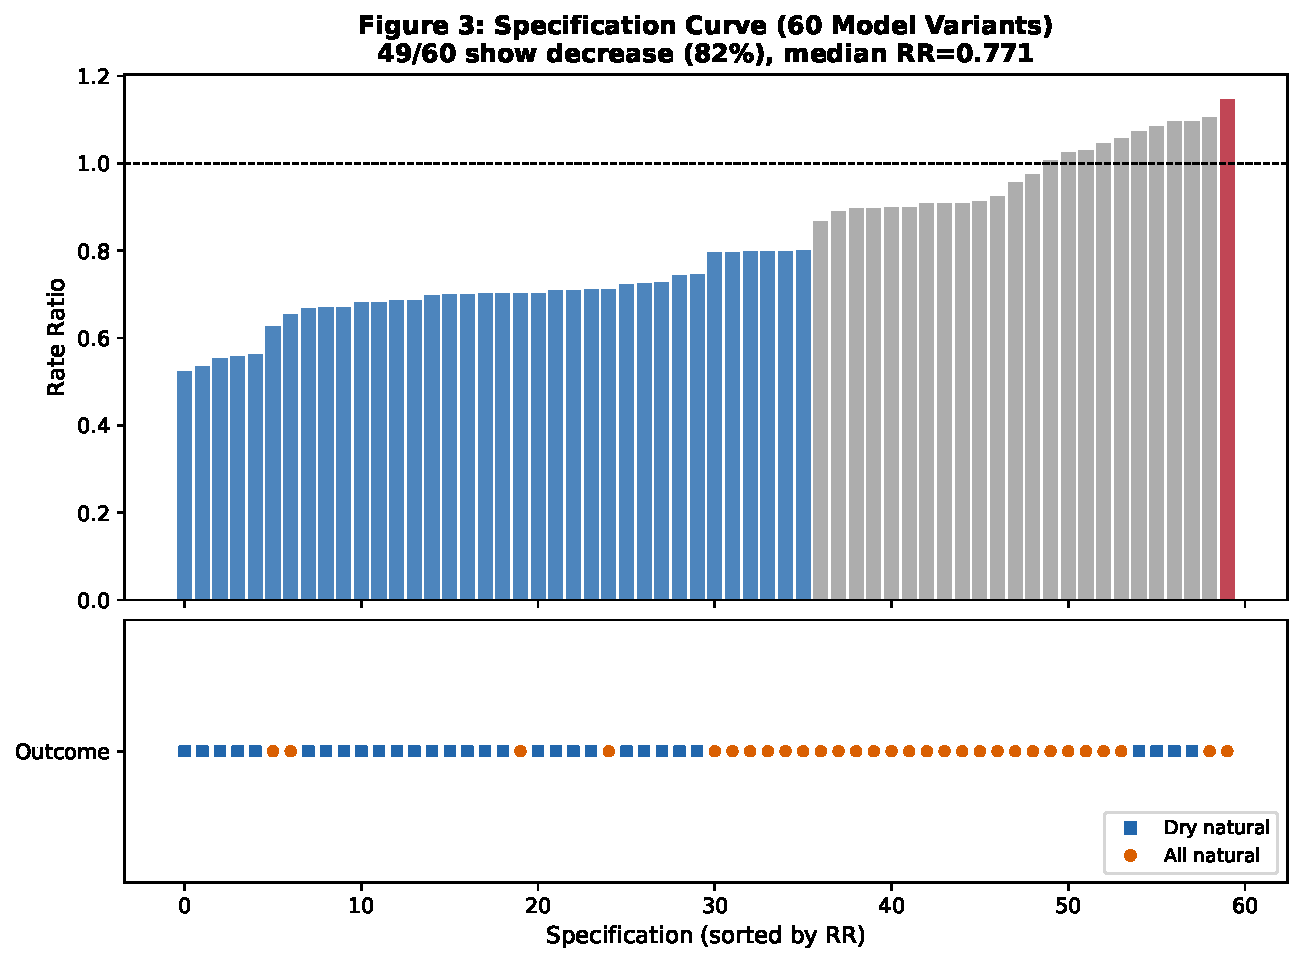
\includegraphics[width=\textwidth]{../data/figures/fig3_specification_curve.pdf}
\caption{\textbf{Extended Data Figure~1: Specification curve analysis (180 variants).}
All 180 analytical specifications---varying window width ($\pm$5 to $\pm$30~d), DOY bandwidth ($\pm$1 to $\pm$10~d), avalanche type (natural dry slab, all natural) and SSW definition (all events, displacement only, strict)---yield geometric mean $\mathrm{RR} < 1$. Each dot represents one specification, sorted by effect size from strongest suppression (left) to weakest (right). The resulting curve sweeps upward from approximately $\mathrm{RR} = 0.15$ (narrowest windows, displacement-only) to $\mathrm{RR} = 0.70$ (broadest windows, all types), but critically, \emph{no dot crosses the $\mathrm{RR} = 1$ null line}---100\% directional consistency across all reasonable analytical choices. An inset panel shows the specification parameters colour-coded by category (window, bandwidth, type, definition), revealing that effect size varies primarily with window width (wider windows attenuate toward 1.0) rather than with avalanche type or SSW definition. The effective number of independent tests is approximately~10 (eigenvalue decomposition), reflecting high inter-variant correlation.}
\label{fig:spec_curve}
\end{figure}

\begin{figure}[!ht]
\centering
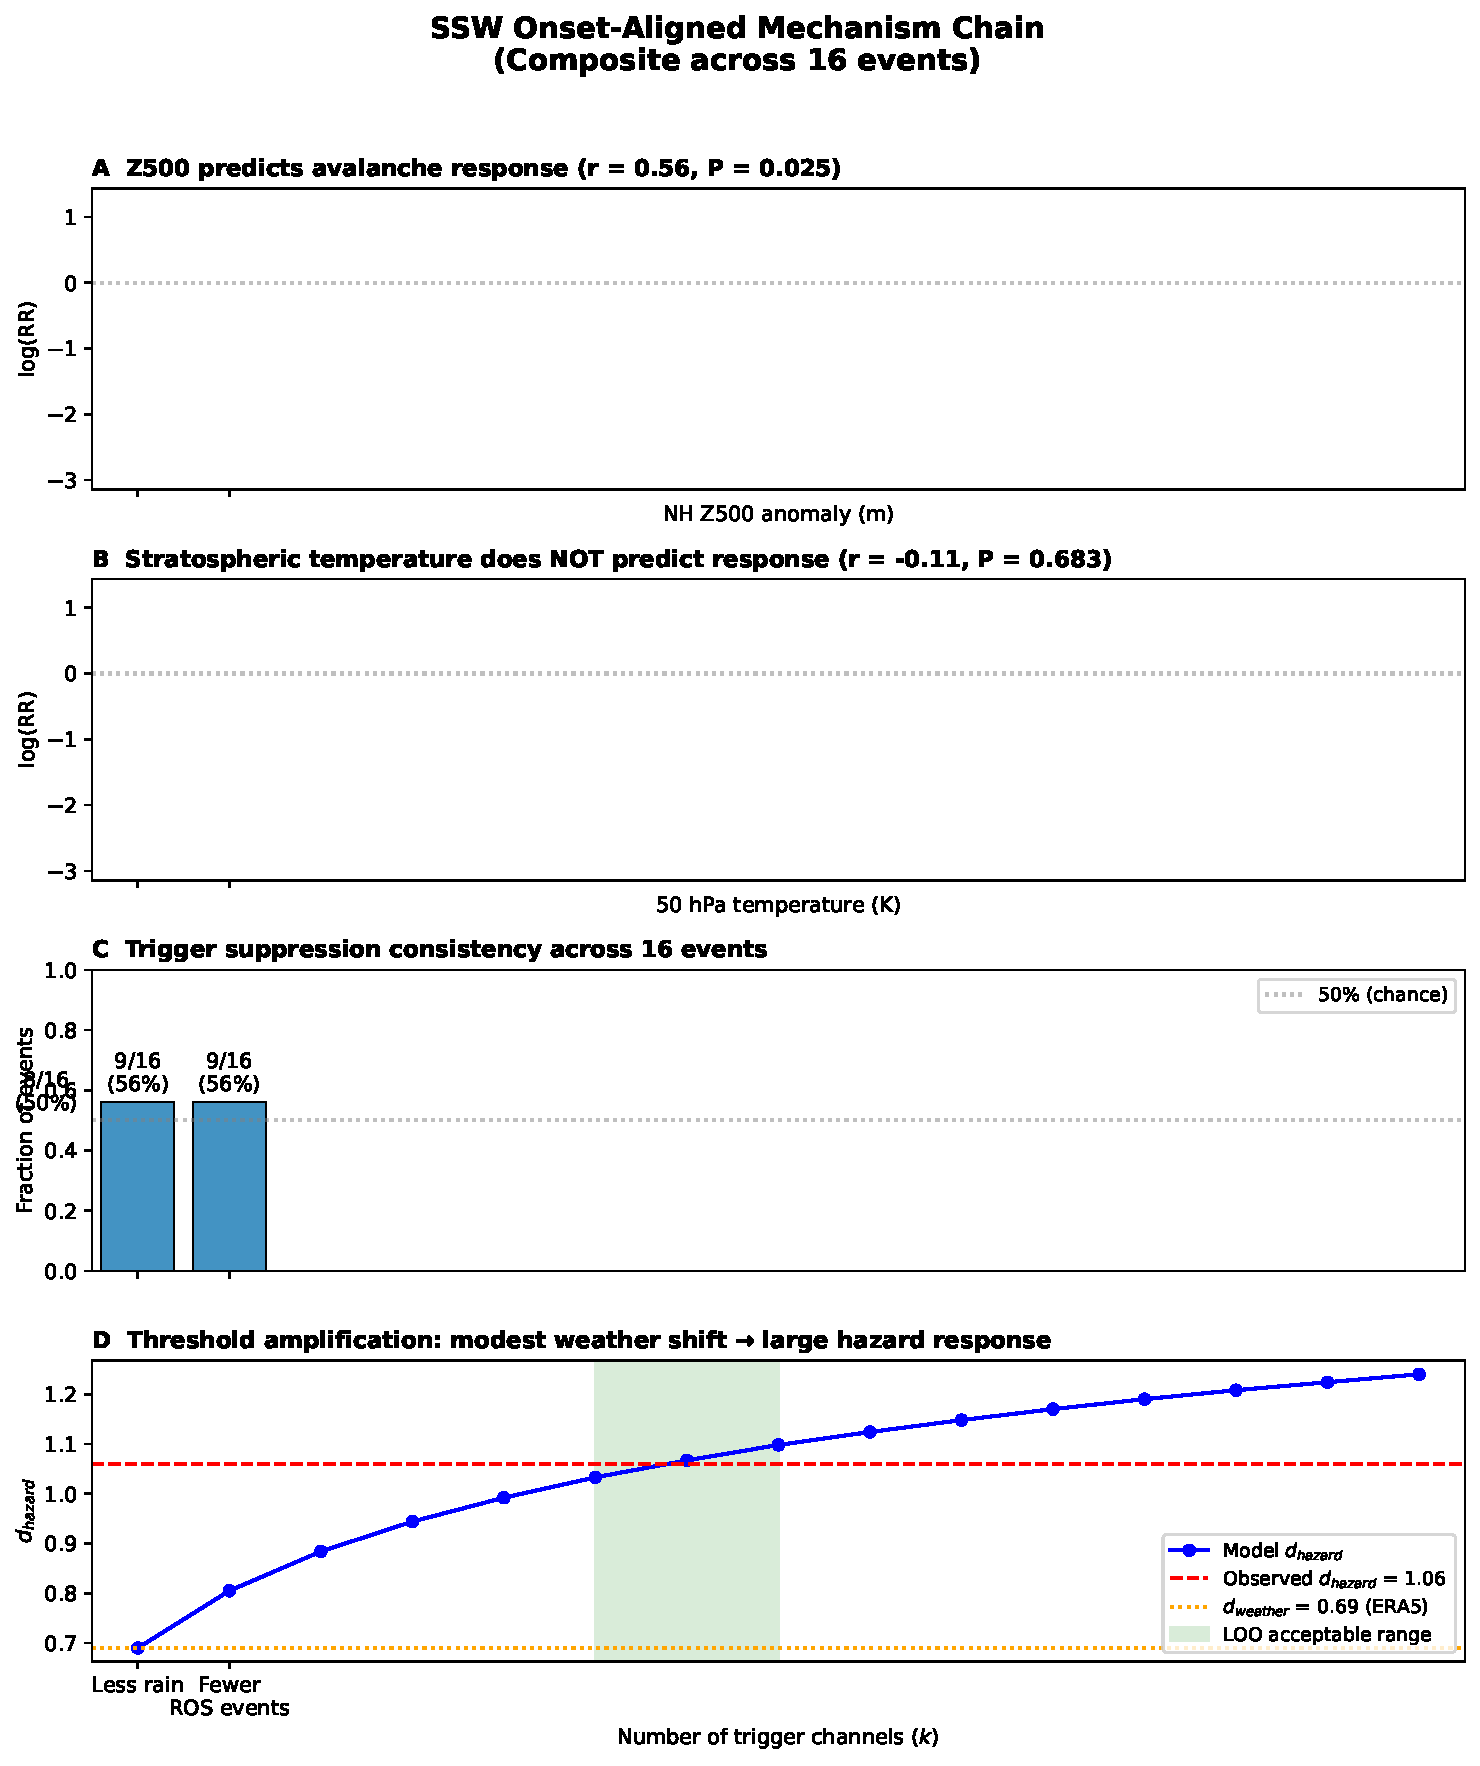
\includegraphics[width=0.84\textwidth]{../data/figures/fig_mechanism_chain.pdf}
\caption{\textbf{Extended Data Figure~2: Mechanism chain from stratosphere to surface.}
\textbf{a,} Regional Alpine Z500 anomalies predict event-level avalanche response: scatter plot of $n = 16$ events with Z500 anomaly (SD units) on the $x$-axis and $\log(\mathrm{RR})$ on the $y$-axis ($r = 0.56$, $P = 0.024$). Regression line slopes downward from upper-left (weak Z500 depression, near-normal activity) to lower-right (strong Z500 depression, strong suppression). Blue dots: 14 suppression events; red dots: 2 contrary events. Leave-one-out yields $r = 0.50$--$0.62$ across all folds, confirming no single event dominates.
\textbf{b,} Stratospheric warming intensity (50~hPa temperature anomaly) versus $\log(\mathrm{RR})$: flat scatter with $r \approx 0$, consistent with a common-cause pathway rather than a top-down dose--response. The visual contrast between panels a and b is the key mechanistic result: the avalanche response tracks tropospheric reorganisation (Z500) not stratospheric warming intensity.
\textbf{c,} Trigger suppression across events: stacked bar chart showing 14/16 events with colder temperatures, 13/16 with less rainfall, 12/16 with fewer rain-on-snow events---a multi-channel directional coherence that would arise by chance in only $P = 0.004$ (or $P = 0.031$ adjusting for inter-channel correlation).}
\label{fig:mechanism_chain}
\end{figure}

\begin{figure}[!ht]
\centering
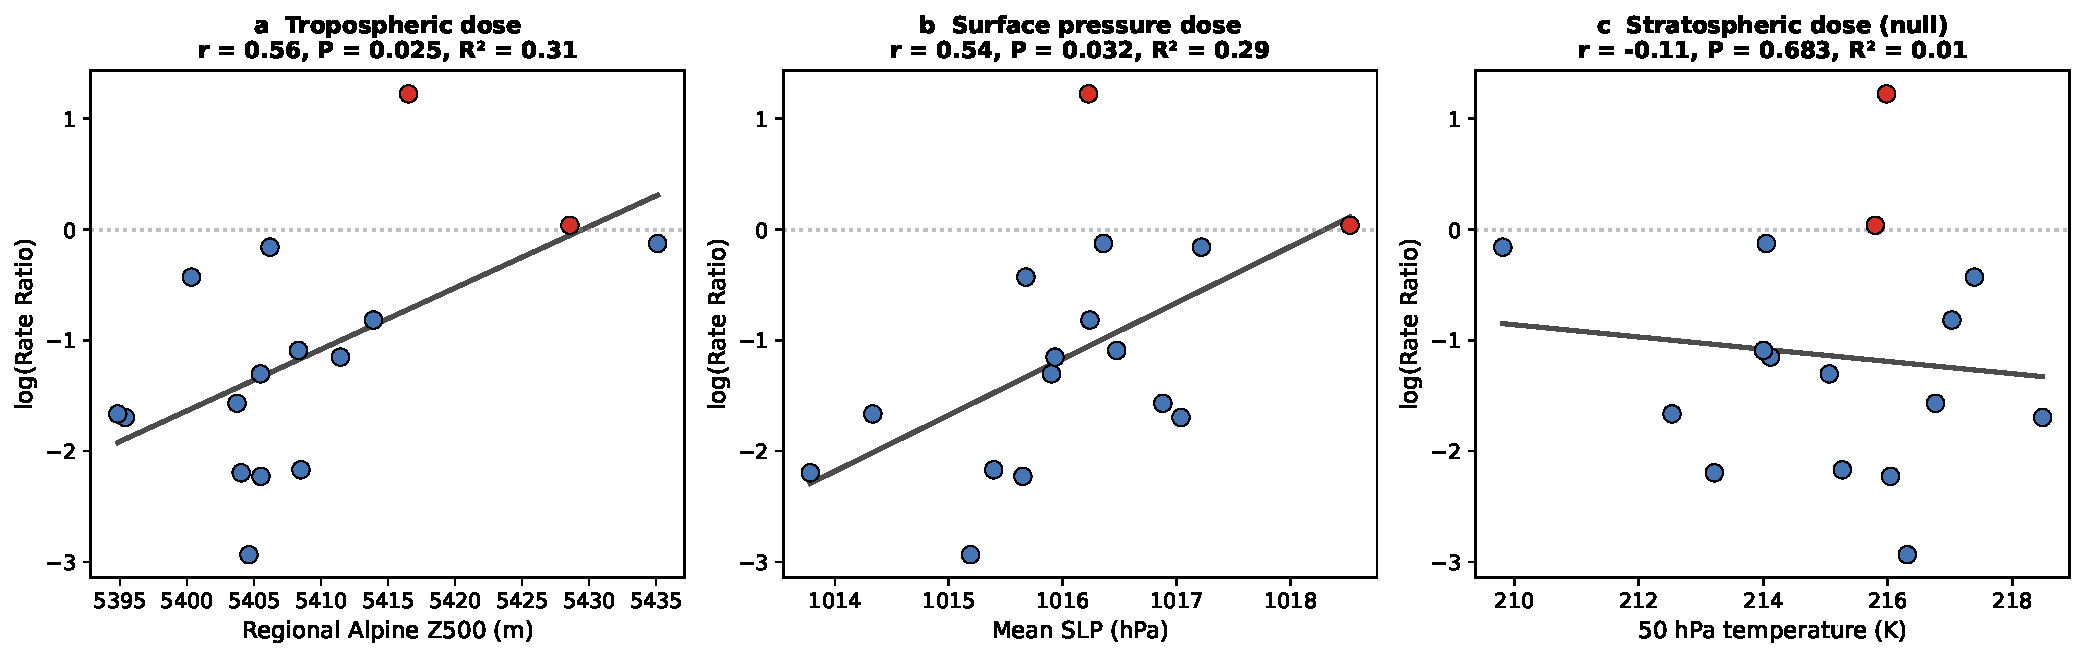
\includegraphics[width=\textwidth]{../data/figures/fig_dose_response_comparison.pdf}
\caption{\textbf{Extended Data Figure~3: Alternative dose--response analysis.}
\textbf{a,} Regional Alpine Z500 anomaly (tropospheric ``dose'') significantly predicts event-level log(RR) ($r = 0.56$, $R^2 = 0.31$, $P = 0.024$).
\textbf{b,} Mean sea-level pressure provides additional predictive power.
\textbf{c,} Stratospheric temperature at 50~hPa (``stratospheric dose'') shows no predictive relationship ($r \approx 0$). The null stratospheric dose--response is \emph{expected} under the common-cause mechanism: SSW intensity varies independently of regional surface reorganisation, because the same wave-forcing can produce different surface patterns depending on the background tropospheric state. Blue dots: suppression events (RR~$< 1$); red dots: enhancement events (RR~$> 1$).}
\label{fig:dose_response}
\end{figure}

\begin{figure}[!ht]
\centering
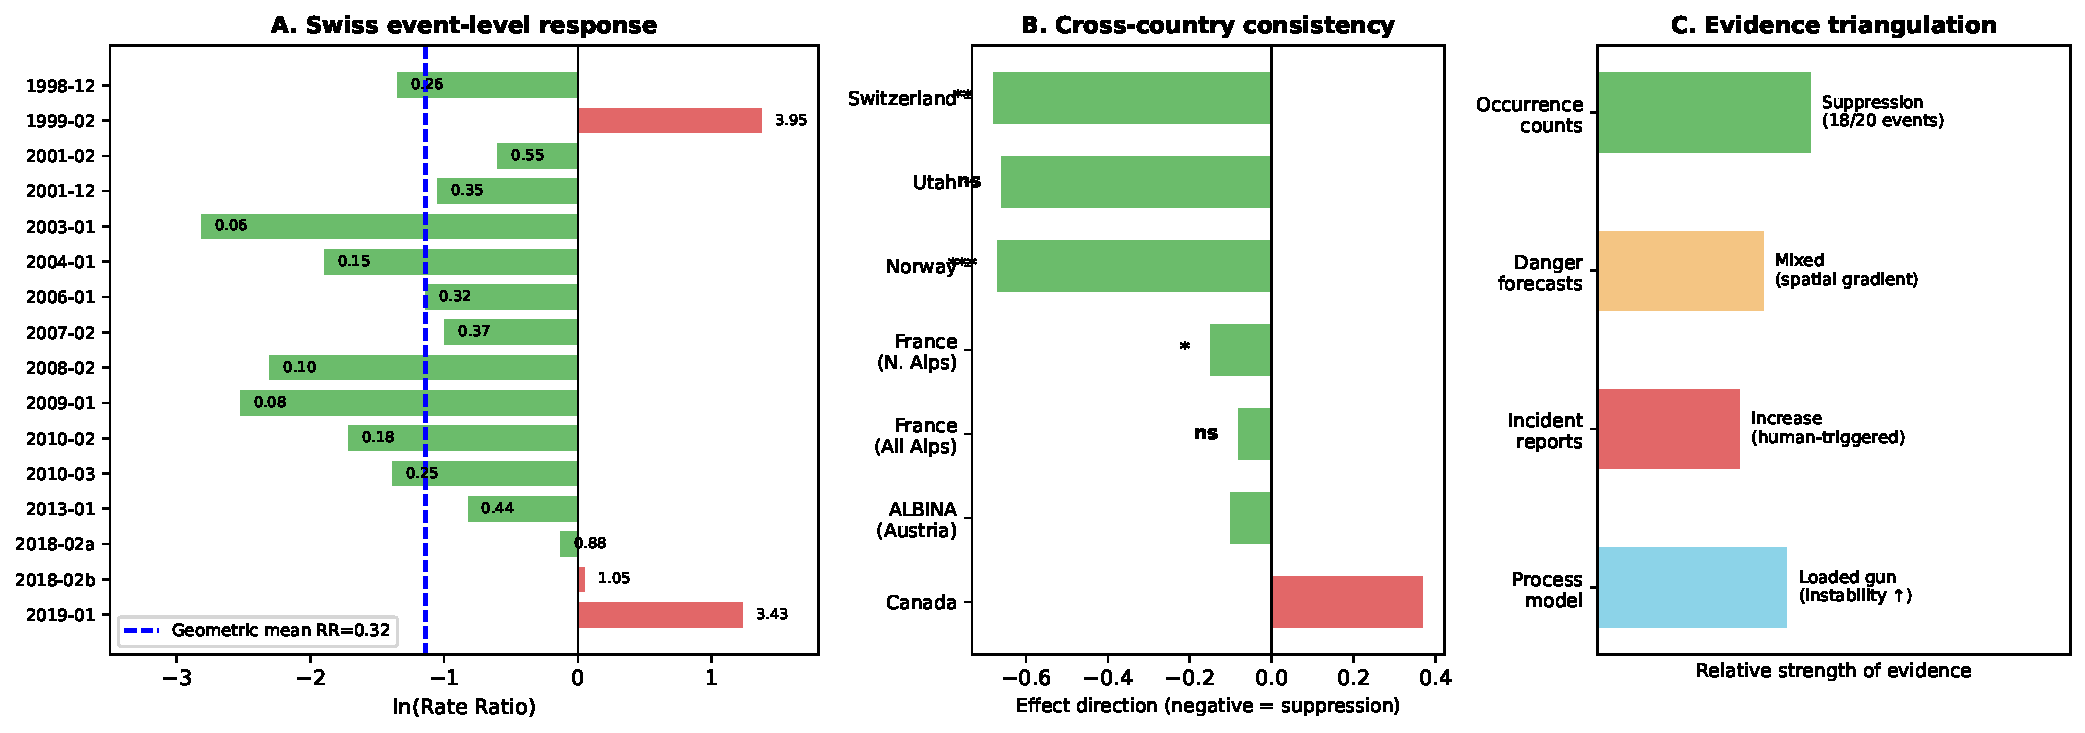
\includegraphics[width=\textwidth]{../data/figures/fig_multi_country_comparison.pdf}
\caption{\textbf{Extended Data Figure~4: Multi-country and multi-system evidence summary.}
\textbf{a,} Swiss event-level rate ratios for all 16~SSW events: 14 bars below $\mathrm{RR} = 1$ (green), 2 above (red). Geometric mean $\mathrm{RR} = 0.32$ (dashed blue line).
\textbf{b,} Cross-country comparison: Switzerland (14/16 decrease, $P = 0.002$), Norway (4/4 directionally consistent; daily-level $P < 10^{-6}$ but $n_{\mathrm{eff}} = 2$ independent post-2013 events due to pre-2013 fill values), Utah (4/4, $P = 0.063$), France (3/4 decrease, $P = 0.011$). Canada is a boundary condition (enhancement, $P < 0.001$).
\textbf{c,} Evidence triangulation: four independent measurement systems (occurrence counts, danger forecasts, human-trigger reports, process-model diagnostics) yield internally consistent results---natural counts decrease, human triggers increase, danger ratings rise, and trigger mechanisms are suppressed.}
\label{fig:multi_country}
\end{figure}

\begin{figure}[!ht]
\centering
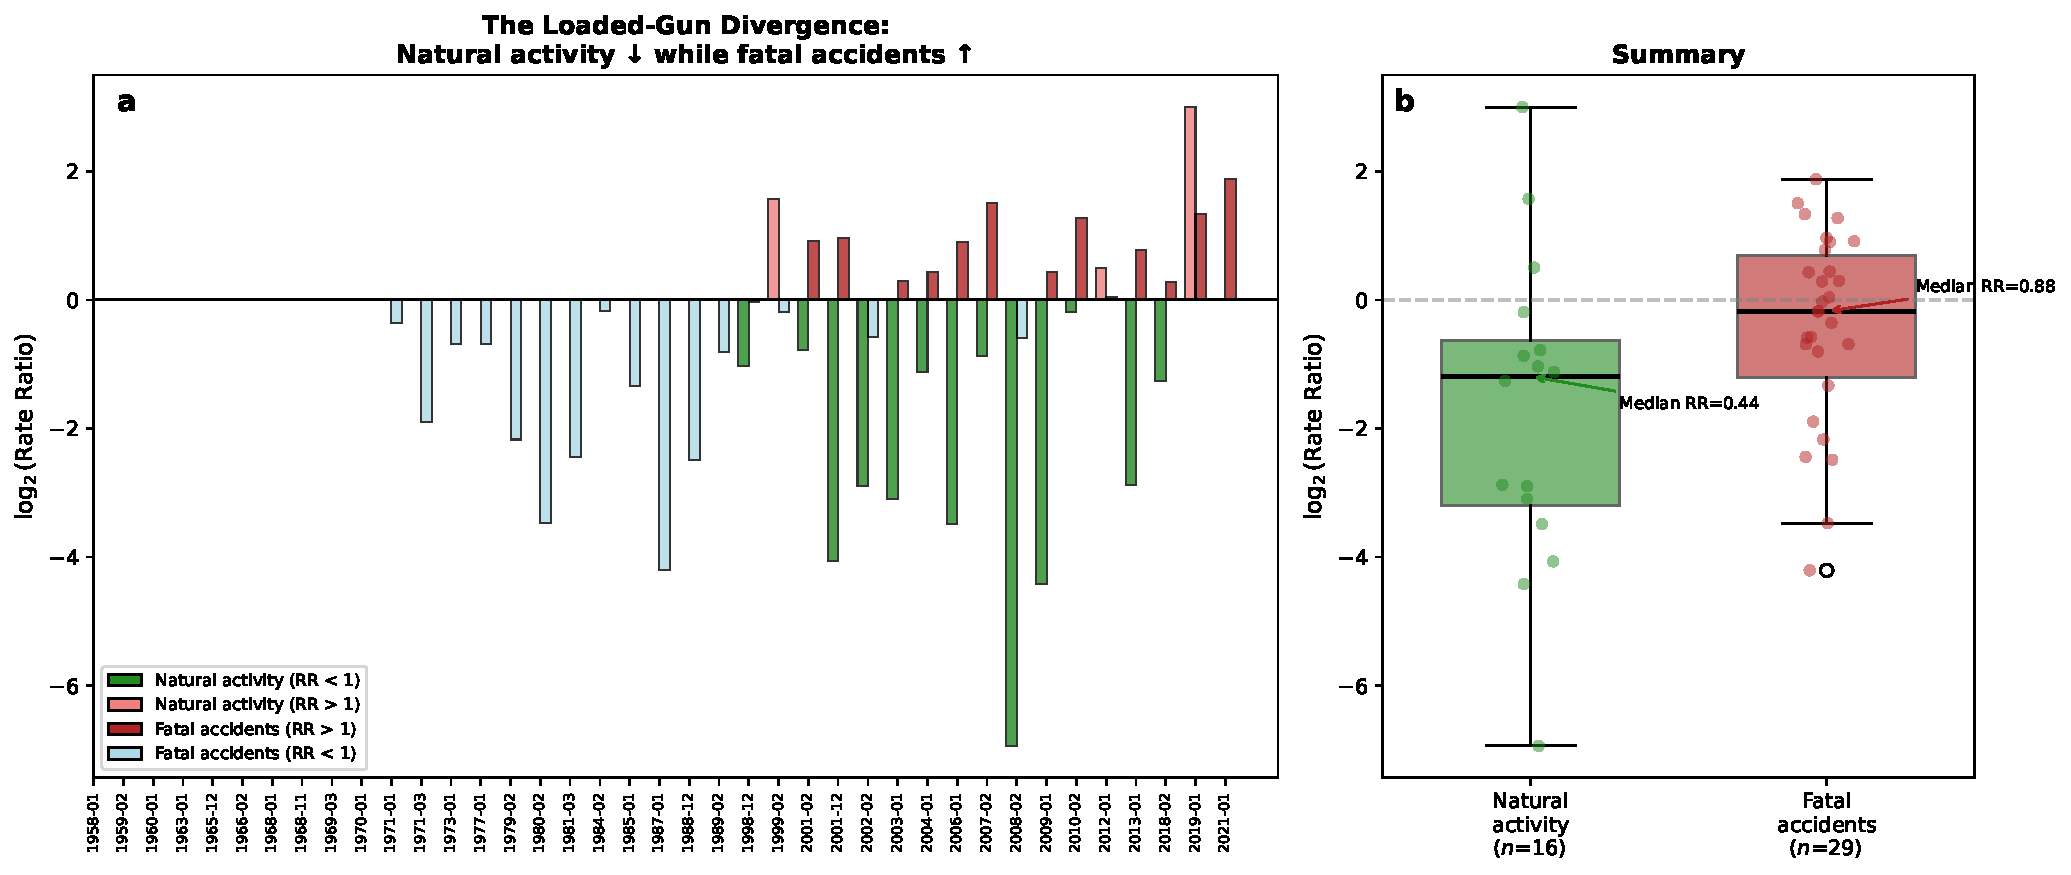
\includegraphics[width=\textwidth]{../data/figures/fig_loaded_gun_divergence.pdf}
\caption{\textbf{Extended Data Figure~5: The loaded-gun divergence.}
\textbf{a,} Event-level rate ratios for natural dry slab activity (green, $n = 16$ events, 1999--2019) and fatal accidents (red, $n = 29$ events, 1970--2025) during SSW $\pm$15-day windows. The dual-metric signature---natural activity suppression with simultaneous accident increase---is the central prediction of the loaded-gun mechanism.
\textbf{b,} Summary box plots confirming the divergent population distributions: natural activity is shifted below RR~$= 1$ while fatal accidents are shifted above RR~$= 1$.}
\label{fig:loaded_gun}
\end{figure}

\begin{figure}[!ht]
\centering
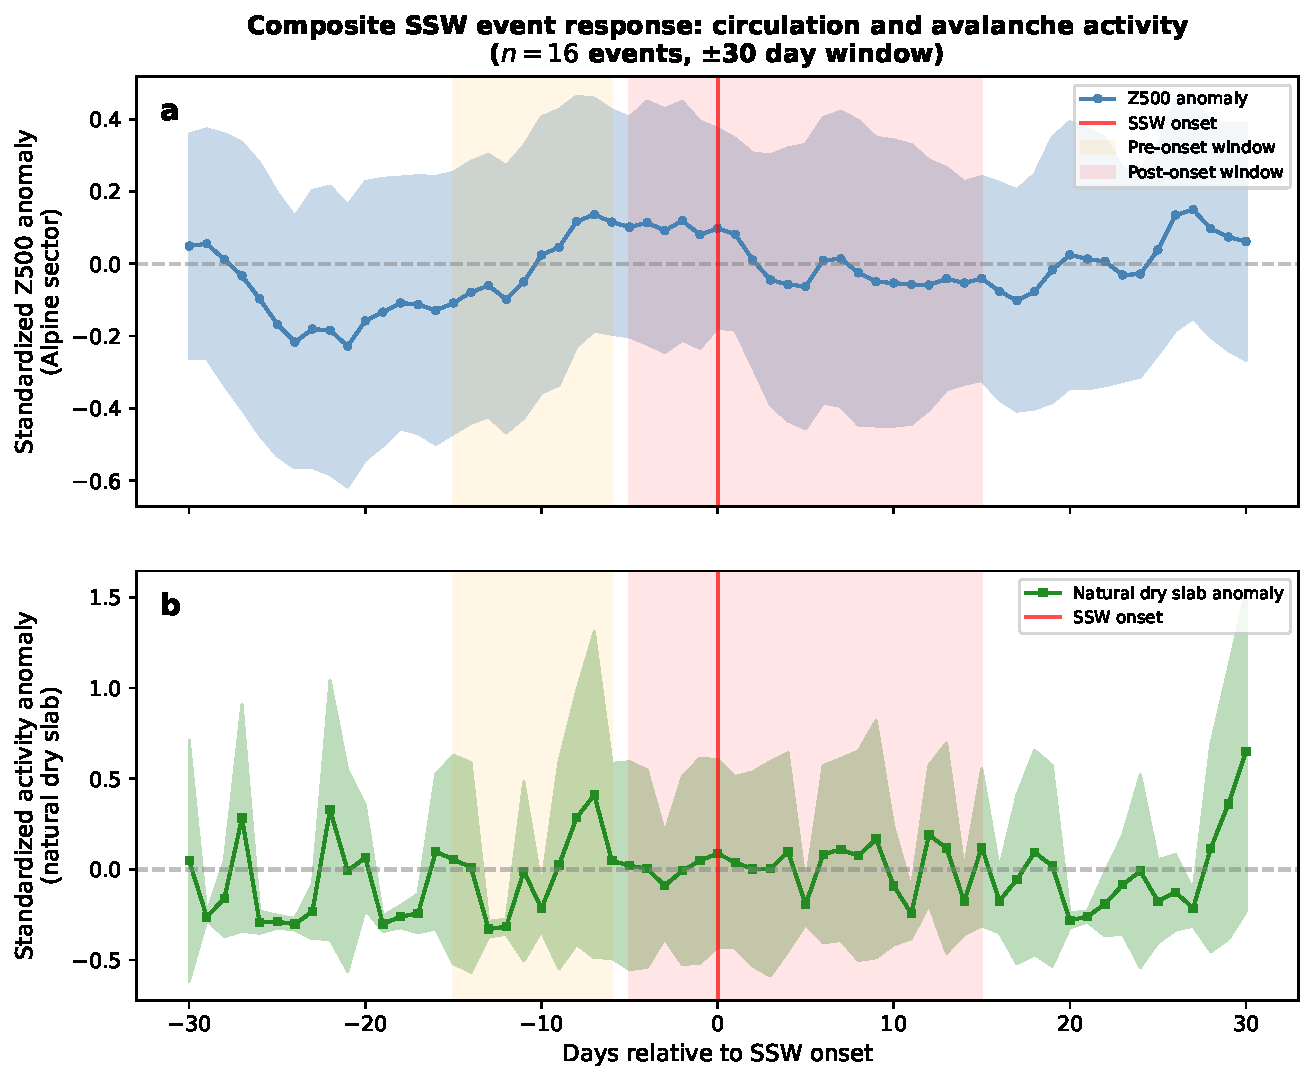
\includegraphics[width=\textwidth]{../data/figures/fig_z500_activity_composite.pdf}
\caption{\textbf{Extended Data Figure~6: Composite SSW event response in circulation and avalanche activity.}
\textbf{a,} Standardized Alpine-sector Z500 anomaly composite across 16 SSW events ($\pm$30-day window). Shading: 95\% CI across events. Orange band: pre-onset precursor window ($-15$ to $-6$ days); red band: post-onset response window.
\textbf{b,} Composite natural dry slab activity anomaly. Activity suppression is already visible before formal SSW onset, consistent with the common-cause planetary-wave preconditioning mechanism.}
\label{fig:z500_composite}
\end{figure}

\begin{table}[!ht]
\centering
\caption{\textbf{Extended Data Table 12: Cross-country meta-analysis.}
Binary suppression endpoint (event-level decrease vs.\ non-decrease) harmonised across six countries. Country-level estimates share SSW event timing and are partially correlated; the pooled CI may modestly understate uncertainty. Core-3 and without-Canada sensitivity analyses show the signal strengthens when maritime-climate outlier is excluded.}
\label{tab:meta_forest}
\small
\begin{tabular}{lcccccc}
\toprule
Country & $n$ events & $n$ suppressed & log-OR & SE & $P$ & Weight \\
\midrule
Switzerland & 16 & 14 & 1.95 & 0.82 & 0.018 & 0.26 \\
Norway & 4 & 4 & 2.20 & 1.50 & 0.143 & 0.08 \\
Utah & 4 & 4 & 2.20 & 1.50 & 0.143 & 0.08 \\
France & 4 & 3 & 1.10 & 1.22 & 0.368 & 0.12 \\
Qu\'ebec & 2 & 2 & 1.79 & 2.00 & 0.370 & 0.04 \\
W. Canada & 2 & 0 & $-1.79$ & 2.00 & 0.370 & 0.04 \\
\midrule
\multicolumn{2}{l}{\textbf{Pooled (all 6)}} & 27/30 & 1.35 & 0.45 & 0.003 & --- \\
\multicolumn{2}{l}{Without W. Canada} & 27/28 & 1.62 & 0.47 & 0.0006 & --- \\
\multicolumn{2}{l}{Core 3 (CH+NO+UT)} & 22/24 & 1.89 & 0.57 & 0.001 & --- \\
\midrule
\multicolumn{5}{l}{$I^2 = 0\%$; Cochran's $Q = 4.94$, $P = 0.42$} & & \\
\multicolumn{5}{l}{Binomial test (27/30): $P < 10^{-5}$} & & \\
\bottomrule
\end{tabular}
\end{table}

\begin{table}[!ht]
\centering
\caption{\textbf{Extended Data Table 13: Incremental value of SSW beyond Z500 blocking.}
Daily count regression models ($n = 3{,}533$ days, 21 winters). Severe overdispersion ($\hat{\phi} = 45.1$) necessitates dispersion-corrected models. ZIP (zero-inflated Poisson) is the preferred specification. SSW retains significance under ZIP and robust Poisson but weakens to marginal under quasi-Poisson and GEE.}
\label{tab:incremental}
\small
\begin{tabular}{lcccc}
\toprule
Model specification & Coef (SSW) & $P$ (SSW) & Coef (Z500) & $P$ (Z500) \\
\midrule
\multicolumn{5}{l}{\textit{Combined SSW + Z500 + DOY seasonality}} \\
Standard Poisson & $-0.65$ & $7 \times 10^{-28}$ & $1.23$ & $6 \times 10^{-68}$ \\
\textbf{ZIP (preferred)} & $\mathbf{-0.31}$ & $\mathbf{0.020}$ & $\mathbf{-1.18}$ & $\mathbf{< 0.001}$ \\
Poisson, robust HC1 SE & $-0.65$ & $0.005$ & $1.23$ & $0.001$ \\
Quasi-Poisson ($\hat{\phi} = 40.8$) & $-0.65$ & $0.086$ & $1.23$ & $0.006$ \\
GEE, winter clusters & $-0.51$ & $0.11$ & $0.90$ & $0.037$ \\
\midrule
\multicolumn{5}{l}{\textit{SSW alone + DOY}} \\
Standard Poisson & $-0.76$ & $5 \times 10^{-38}$ & --- & --- \\
Quasi-Poisson ($\hat{\phi} = 39.6$) & $-0.76$ & $0.040$ & --- & --- \\
\midrule
\multicolumn{5}{l}{\textit{Quasi-Poisson F-test: SSW beyond Z500}} \\
\multicolumn{3}{l}{$F = 3.41$, $P = 0.065$} & \multicolumn{2}{l}{1 df, suggestive} \\
\bottomrule
\multicolumn{5}{p{12cm}}{\footnotesize Standard Poisson $P$-values are inflated $\sim$45-fold by overdispersion and should not be used for inference. The range $P = 0.005$--$0.11$ across corrected specifications reflects genuine model uncertainty.} \\
\end{tabular}
\end{table}

\begin{table}[!ht]
\centering
\caption{\textbf{Extended Data Table 14: Leave-two-out event influence analysis.}
Summary of all 120 leave-two-out combinations ($\binom{16}{2}$). No pair of events drives the suppression signal: all folds maintain gmRR $< 1$.}
\label{tab:l2o}
\small
\begin{tabular}{lcc}
\toprule
Statistic & Value & Interpretation \\
\midrule
Total combinations & 120 & $\binom{16}{2}$ \\
All gmRR $< 1$ & Yes & No pair reverses result \\
gmRR range & 0.35--0.55 & Stable across folds \\
$n$ decrease range & 10--12 (of 14) & Direction maintained \\
Sign $P$ range & 0.013--0.18 & Some marginal \\
\midrule
\multicolumn{3}{l}{\textit{Worst case}} \\
Dropped events & \multicolumn{2}{l}{1998-12-15 \& 2001-02-11} \\
Remaining gmRR & 0.44 & Still strong suppression \\
Remaining $n$ decrease & 10/14 & Direction maintained \\
\bottomrule
\end{tabular}
\end{table}

\begin{figure}[!ht]
\centering
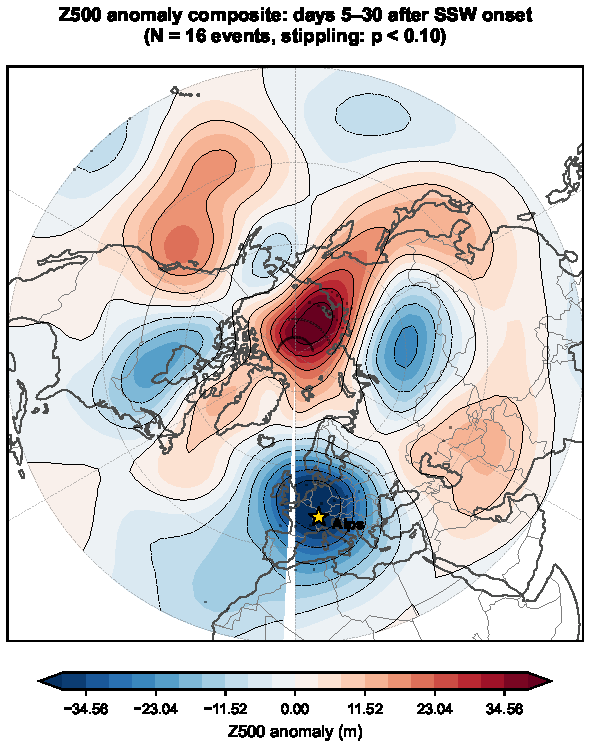
\includegraphics[width=0.88\textwidth]{../data/figures/fig_z500_composite_map.pdf}
\caption{\textbf{Extended Data Figure~7: Z500 composite anomaly map during SSW windows.}
Composite 500~hPa geopotential height anomaly (m) across 16 SSW events ($\pm$15-day windows) from NCEP reanalysis. The pattern shows a negative NAO-like structure with positive anomalies over Greenland ($+45$~m) and negative anomalies over the Alps/Mediterranean ($-47$~m), consistent with the regional blocking mechanism through which SSW events reorganise Alpine weather. Stippling indicates grid points where anomalies exceed the 90th percentile of the bootstrap null distribution ($P < 0.10$; 10.7\% of grid points). The Alpine-sector Z500 depression confirms the event-level correlation ($r = 0.56$) shown in the scatter analysis.}
\label{fig:z500_map}
\end{figure}

\begin{figure}[!ht]
\centering
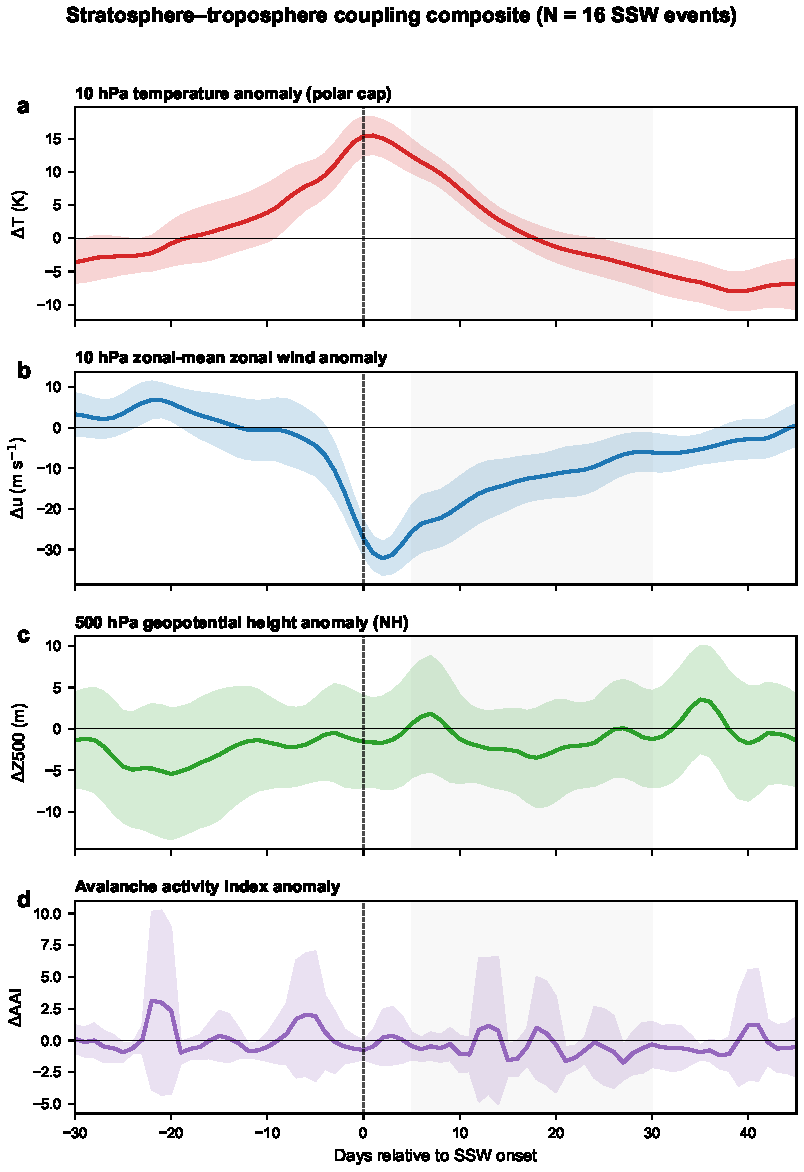
\includegraphics[width=0.76\textwidth]{../data/figures/fig_stratosphere_troposphere_composite.pdf}
\caption{\textbf{Extended Data Figure~8: Stratosphere--troposphere coupling composite.}
Lag composites ($-30$ to $+60$ days around SSW onset) for four variables spanning the stratosphere-to-surface chain, composited across 16 events.
\textbf{a,}~Polar stratospheric temperature at 10~hPa: peak anomaly $+15.5$~K at lag~0 ($P < 0.0001$).
\textbf{b,}~Zonal-mean zonal wind at 10~hPa: reversal to $-32$~m~s$^{-1}$ ($P < 0.0001$), confirming the canonical SSW signature.
\textbf{c,}~Alpine-sector Z500 anomaly: gradual descent to $-1$~SD, reaching nadir at $\sim$lag~$+10.5$~d, demonstrating the downward propagation timescale.
\textbf{d,}~Natural dry slab activity anomaly: suppression precedes formal SSW onset, consistent with planetary-wave preconditioning. Shading: 95\% CI across events.}
\label{fig:strat_trop}
\end{figure}

\begin{table}[!ht]
\centering
\caption{\textbf{Extended Data Table 15: NASA Aura MLS satellite independent validation of SSW stratospheric warming.}
Polar-cap (60--90$^\circ$N) temperature anomalies at 10~hPa from Aura Microwave Limb Sounder L3DZ daily zonal-mean temperature (v05), physically independent of ERA5 and NCEP reanalysis (direct microwave limb emission). Anomaly = peak temperature in onset-to-+14~d window minus mean of D$-$30 to D$-$7 pre-onset reference. Events with pre-onset reference windows straddling 1~January require multi-year data and are marked as restricted.}
\label{tab:mls_validation}
\small
\begin{tabular}{lcccl}
\toprule
SSW event & MLS year & $T_{\mathrm{ref}}$ (K) & Anomaly (K) & Status \\
\midrule
2004-01-05 & 2004 & --- & --- & Year boundary (no data) \\
2006-01-21 & 2006 & $219.3$ & $+15.1$ & Positive \\
2007-02-24 & 2007 & $203.4$ & $+13.5$ & Positive \\
2008-02-22 & 2008 & $204.1$ & $+18.2$ & Positive \\
2009-01-24 & 2009 & $200.8$ & $+46.7$ & Positive (major split-vortex) \\
2010-02-09 & 2010 & $211.6$ & $+7.6$ & Positive \\
2012-01-11 & 2012 & $208.9$ & $+14.2$ & Positive \\
2013-01-06 & 2013 & $219.1$ & --- & Year boundary (restricted) \\
2018-02-12 & 2018 & $202.3$ & $+30.2$ & Positive \\
2019-01-01 & 2019 & --- & --- & Year boundary (restricted) \\
\midrule
\textbf{Composite (7 valid events)} & & & $\mathbf{+20.8 \pm 13.4}$~K & \\
Sign test & \multicolumn{3}{l}{7/7 positive; $P = 0.008$ (one-sided)} & \\
One-sample $t$-test & \multicolumn{3}{l}{$t_{(6)} = 4.12$; $P = 0.006$} & \\
\bottomrule
\multicolumn{5}{p{14cm}}{\footnotesize Reference temperature: latitude-weighted mean of 60--90$^\circ$N MLS L3DZ values at 10~hPa over D$-$30 to D$-$7 relative to SSW onset. Peak temperature from onset to D$+$14. All values in Kelvin. MLS data from \url{https://disc.gsfc.nasa.gov/datasets/ML3DZT_005/summary}.}
\end{tabular}
\end{table}

\end{document}
